% This is the basic latex structure to include the flyleaf. It is up to you to either \input the file and compile it with your main latex files or to generate a pdf and add it to your project. However this is a simple flyleaf since my university only had a template for word. You can use it and change it 
\RequirePackage{silence} % :-\
\WarningFilter{scrreprt}{Usage of package `titlesec'}
%\WarningFilter{scrreprt}{Activating an ugly workaround}
\WarningFilter{titlesec}{Non standard sectioning command detected}

\documentclass[12pt,a4paper,bibliography=totocnumbered,listof=totocnumbered]{report}
\usepackage[utf8]{inputenc}
\usepackage{epsfig}		% needed to import epf files
\usepackage{lipsum}		% needed to generate blindtext
\usepackage{amssymb}
\usepackage{amsmath}
\usepackage{listings}
\usepackage{graphicx}
\usepackage{array}
\usepackage{hyperref}


%\newgeometry{
%	top=2.5cm,
%	bottom=2.35cm,
%	inner=2.25cm,
%	outer=2.15cm,
%}


% ****************************************************************************************************
% classicthesis-config.tex
% formerly known as loadpackages.sty, classicthesis-ldpkg.sty, and classicthesis-preamble.sty
% Use it at the beginning of your ClassicThesis.tex, or as a LaTeX Preamble
% in your ClassicThesis.{tex,lyx} with % ****************************************************************************************************
% classicthesis-config.tex
% formerly known as loadpackages.sty, classicthesis-ldpkg.sty, and classicthesis-preamble.sty
% Use it at the beginning of your ClassicThesis.tex, or as a LaTeX Preamble
% in your ClassicThesis.{tex,lyx} with % ****************************************************************************************************
% classicthesis-config.tex
% formerly known as loadpackages.sty, classicthesis-ldpkg.sty, and classicthesis-preamble.sty
% Use it at the beginning of your ClassicThesis.tex, or as a LaTeX Preamble
% in your ClassicThesis.{tex,lyx} with \input{classicthesis-config}
% ****************************************************************************************************
% If you like the classicthesis, then I would appreciate a postcard.
% My address can be found in the file ClassicThesis.pdf. A collection
% of the postcards I received so far is available online at
% http://postcards.miede.de
% ****************************************************************************************************

% ********************************************************************
% Setup, finetuning, and useful commands
% ********************************************************************
\newcounter{dummy} % necessary for correct hyperlinks (to index, bib, etc.)
\newlength{\abcd} % for ab..z string length calculation
\providecommand{\mLyX}{L\kern-.1667em\lower.25em\hbox{Y}\kern-.125emX\@}
\newcommand{\ie}{i.\,e.}
\newcommand{\Ie}{I.\,e.}
\newcommand{\eg}{e.\,g.}
\newcommand{\Eg}{E.\,g.}
% ****************************************************************************************************
% ****************************************************************************************************
% If you like the classicthesis, then I would appreciate a postcard.
% My address can be found in the file ClassicThesis.pdf. A collection
% of the postcards I received so far is available online at
% http://postcards.miede.de
% ****************************************************************************************************

% ********************************************************************
% Setup, finetuning, and useful commands
% ********************************************************************
\newcounter{dummy} % necessary for correct hyperlinks (to index, bib, etc.)
\newlength{\abcd} % for ab..z string length calculation
\providecommand{\mLyX}{L\kern-.1667em\lower.25em\hbox{Y}\kern-.125emX\@}
\newcommand{\ie}{i.\,e.}
\newcommand{\Ie}{I.\,e.}
\newcommand{\eg}{e.\,g.}
\newcommand{\Eg}{E.\,g.}
% ****************************************************************************************************
% ****************************************************************************************************
% If you like the classicthesis, then I would appreciate a postcard.
% My address can be found in the file ClassicThesis.pdf. A collection
% of the postcards I received so far is available online at
% http://postcards.miede.de
% ****************************************************************************************************

% ********************************************************************
% Setup, finetuning, and useful commands
% ********************************************************************
\newcounter{dummy} % necessary for correct hyperlinks (to index, bib, etc.)
\newlength{\abcd} % for ab..z string length calculation
\providecommand{\mLyX}{L\kern-.1667em\lower.25em\hbox{Y}\kern-.125emX\@}
\newcommand{\ie}{i.\,e.}
\newcommand{\Ie}{I.\,e.}
\newcommand{\eg}{e.\,g.}
\newcommand{\Eg}{E.\,g.}
% ****************************************************************************************************

\begin{document}
\frenchspacing
\raggedbottom	
\pagenumbering{roman}
\pagestyle{plain}

% Based on the template of Prof. Dr.-Ing. Karl Heinrich Hofmann (https://www.hs-rm.de/de/hochschule/personen/hofmann-karl-heinrich/). 
% Changed by Nils Minor as template for HDA (EIT) in December 2017

\textheight 25 cm                
\textwidth 17 cm
\topmargin -15mm
\parindent 0 ex 			
\parskip 2 ex
\raggedbottom
\oddsidemargin -6.5mm    	
\evensidemargin -16.5mm 
% Page border should be:
% top: 15 mm
% oddside:  left 25 mm, right 15 mm
% evenside: left 15 mm, right 25 mm
%
% Eingaben
\newcommand{\thesis}{Masterthesis}
\newcommand{\writer}{Your Name}
\newcommand{\completiondate}{01.01.1970}
\newcommand{\topic}{ON THE TRACK OF RANDOMNESS FOR AUTOMOTIVE CYBERSECURITY}
\newcommand{\supervisor}{Prof. Dr. First Supervisor}
\newcommand{\supervisorsec}{Prof. Dr. Second Supervisor}
\newcommand{\supervisorindustrial}{Dr. Ing. Industrial Supervisor (Company)}
\newcommand{\supervisorindustrialsec}{Second Supervisor (Company)}
%%%%%%%%%%%%%%%%%%%%%%%%%%%%%%%%%%%%%%%%%%%%%%%%%%%%%%%%%%%%%%%%%%%%%%%%%%%%%%%%%%%%%%
\thispagestyle{empty} 
\vspace{-20mm}
\begin{minipage}[t]{8cm}  

\epsfig{file=flyleaf/eit_logo.png,width=6cm}
\end{minipage}
\hfill
%\raisebox{11.5ex}{\small \begin{tabular}[t]{l}
%{\textbf{Faculty}} \\Electrical Engineering and \\Information Technology International  \\[1ex]
%{\textbf{Major}} \\ Embedded Systems and Microelectronics
%\end{tabular}}
\vspace{30mm}
\begin{center}{\Huge \textbf{\thesis}} \par
\vspace{20mm} \baselineskip 35pt
{\LARGE\textbf  \topic} \par
\vspace{16mm}
{\LARGE\textbf  \writer} \par
\end{center}
% 
\vspace{20mm}
\vfill
\begin{tabular}{lp{382pt}}
Completion date	 		 &  \completiondate \\[5ex]
1st Academic Supervisor:	 &  \supervisor \\[0.5ex]
2nd Academic Supervisor:	 &  \supervisorsec \\[0.5ex]
Industrial Supervisor:	 &  \supervisorindustrial \\ 
					     & 	\supervisorindustrialsec
\end{tabular}
%%%%%%%%%%%%%%%%%%%%%%%%%%%%%%%%%%%%%%%%%%%%%%%%%%%%%%%%%%%%%%%%%%%%%%%%%%%%%%%%%%%%%%
% Empty page
\newpage
\thispagestyle{empty}
\rule[0ex]{0ex}{0ex} 	
%%%%%%%%%%%%%%%%%%%%%%%%%%%%%%%%%%%%%%%%%%%%%%%%%%%%%%%%%%%%%%%%%%%%%%%%%%%%%%%%%%%%%%
\newpage
\thispagestyle{empty} 

\textbf{\Large Student}
\par \vspace{10mm}
\rule[0ex]{0.45\textwidth}{0.4pt} \hspace{14mm}
\rule[0ex]{0.45\textwidth}{0.4pt}\\
First (Given) Name \hspace{55mm}
Last (Family) Name
\par \vspace{10mm}
\rule[0ex]{0.45\textwidth}{0.4pt} \hspace{14mm}
\rule[0ex]{0.45\textwidth}{0.4pt}\\
Date of Birth \hspace{66mm}
Matr.-No.


\par \vspace{10mm}
\rule[0ex]{\textwidth}{0.4pt} \\
1st Academic Supervisor (\textit{\supervisor})
\par \vspace{10mm}
\rule[0ex]{\textwidth}{0.4pt} \\
2st Academic Supervisor (\textit{\supervisorsec})


\par \vspace{15mm} 
In partial fulfillment of the requirements of the \textbf{University of Applied Sciences Hochschule Darmstadt (h\_da)} for the degree \textbf{Master of Science in Electrical Engineering} carried out in collaboration with \textbf{Industrial Enterprise}\\[1ex]

Company: \rule[0ex]{0.885\textwidth}{0.4pt} 

Address: \rule[0ex]{0.9\textwidth}{0.4pt}\\[2ex]
\rule[0ex]{\textwidth}{0.4pt} \\[2ex]
\rule[0ex]{\textwidth}{0.4pt} \\[2ex]
\rule[0ex]{\textwidth}{0.4pt} \\[0ex]
\vspace{1cm}
\begin{table}[h]
	\begin{tabular}{lp{14.7cm}}
		$\square$ & This Master Thesis contains confidential data and may only be made available to the 
	supervisor, the members of the examination board and authorized members of Darmstadt 
	University of Applied Sciences.
	\end{tabular}
\end{table}



\newpage %%%%%%%%%%%%%%%%%%%%%%%%%%%%%%%%%%%%%%%%%%%%%%%%%%%%%%%%%%%%%%%%%%%%%%%%%%%

% Declaration
\newpage
\thispagestyle{empty} 
%

\textbf{\Large Declaration}
\par \vspace{5mm}
I hereby declare that this thesis is a presentation of my original research work and that no other sources were used other than what is cited.
\par
I furthermore declare that wherever contributions of others are involved, this contribution is indicated, clearly acknowledged and due reference is given to the author and source.
\par
I also certify that all content without reference or citation contained in this thesis is original work.
\par
I acknowledge that any misappropriation of the previous declarations can be considered a case of academic fraud.
\par
\vspace{25mm}
\rule[0ex]{\textwidth}{0.4pt}
(Darmstadt / Date)\hspace{30ex}	(Signature student)


\newpage %%%%%%%%%%%%%%%%%%%%%%%%%%%%%%%%%%%%%%%%%%%%%%%%%%%%%%%%%%%%%%%%%%%%%%%%%%%


\section*{Abstract}	% Remove the dot (*) to show the section numbering

Hi Hello
\lipsum[1-2]		% Write here your personal abstract

%%*******************************************************
% Table of Contents
%*******************************************************
%\pagestyle{scrheadings}
%\refstepcounter{dummy}
%\pdfbookmark[1]{\contentsname}{tableofcontents}
%\setcounter{tocdepth}{2} % <-- 2 includes up to subsections in the ToC
%\setcounter{secnumdepth}{3} % <-- 3 numbers up to subsubsections
%\manualmark
%\markboth{\spacedlowsmallcaps{\contentsname}}{\spacedlowsmallcaps{\contentsname}}
\tableofcontents

\cleardoublepage
\listoffigures

\cleardoublepage
%\thispagestyle{empty}
\setcounter{page}{1}
\tableofcontents
\cleardoublepage
\addcontentsline{toc}{chapter}{\listfigurename}
\listoffigures
\cleardoublepage
\addcontentsline{toc}{chapter}{\listtablename}
\listoftables

\newpage
\setcounter{page}{1}
\pagenumbering{arabic}

\chapter{Introduction}
\label{ch:intro}



%
% Section: Motivation
%
\section{Motivation}
\label{sec:intro:structure}

refernce to figure \ref{fig:1:1}

reference to chapter \ref{ch:chapter03}

acronym test \acf{AES}, \acs{AES} and \acp{AES}

citation \cite{RANDOM-1998}


\begin{figure}[htbp]
	\centering
	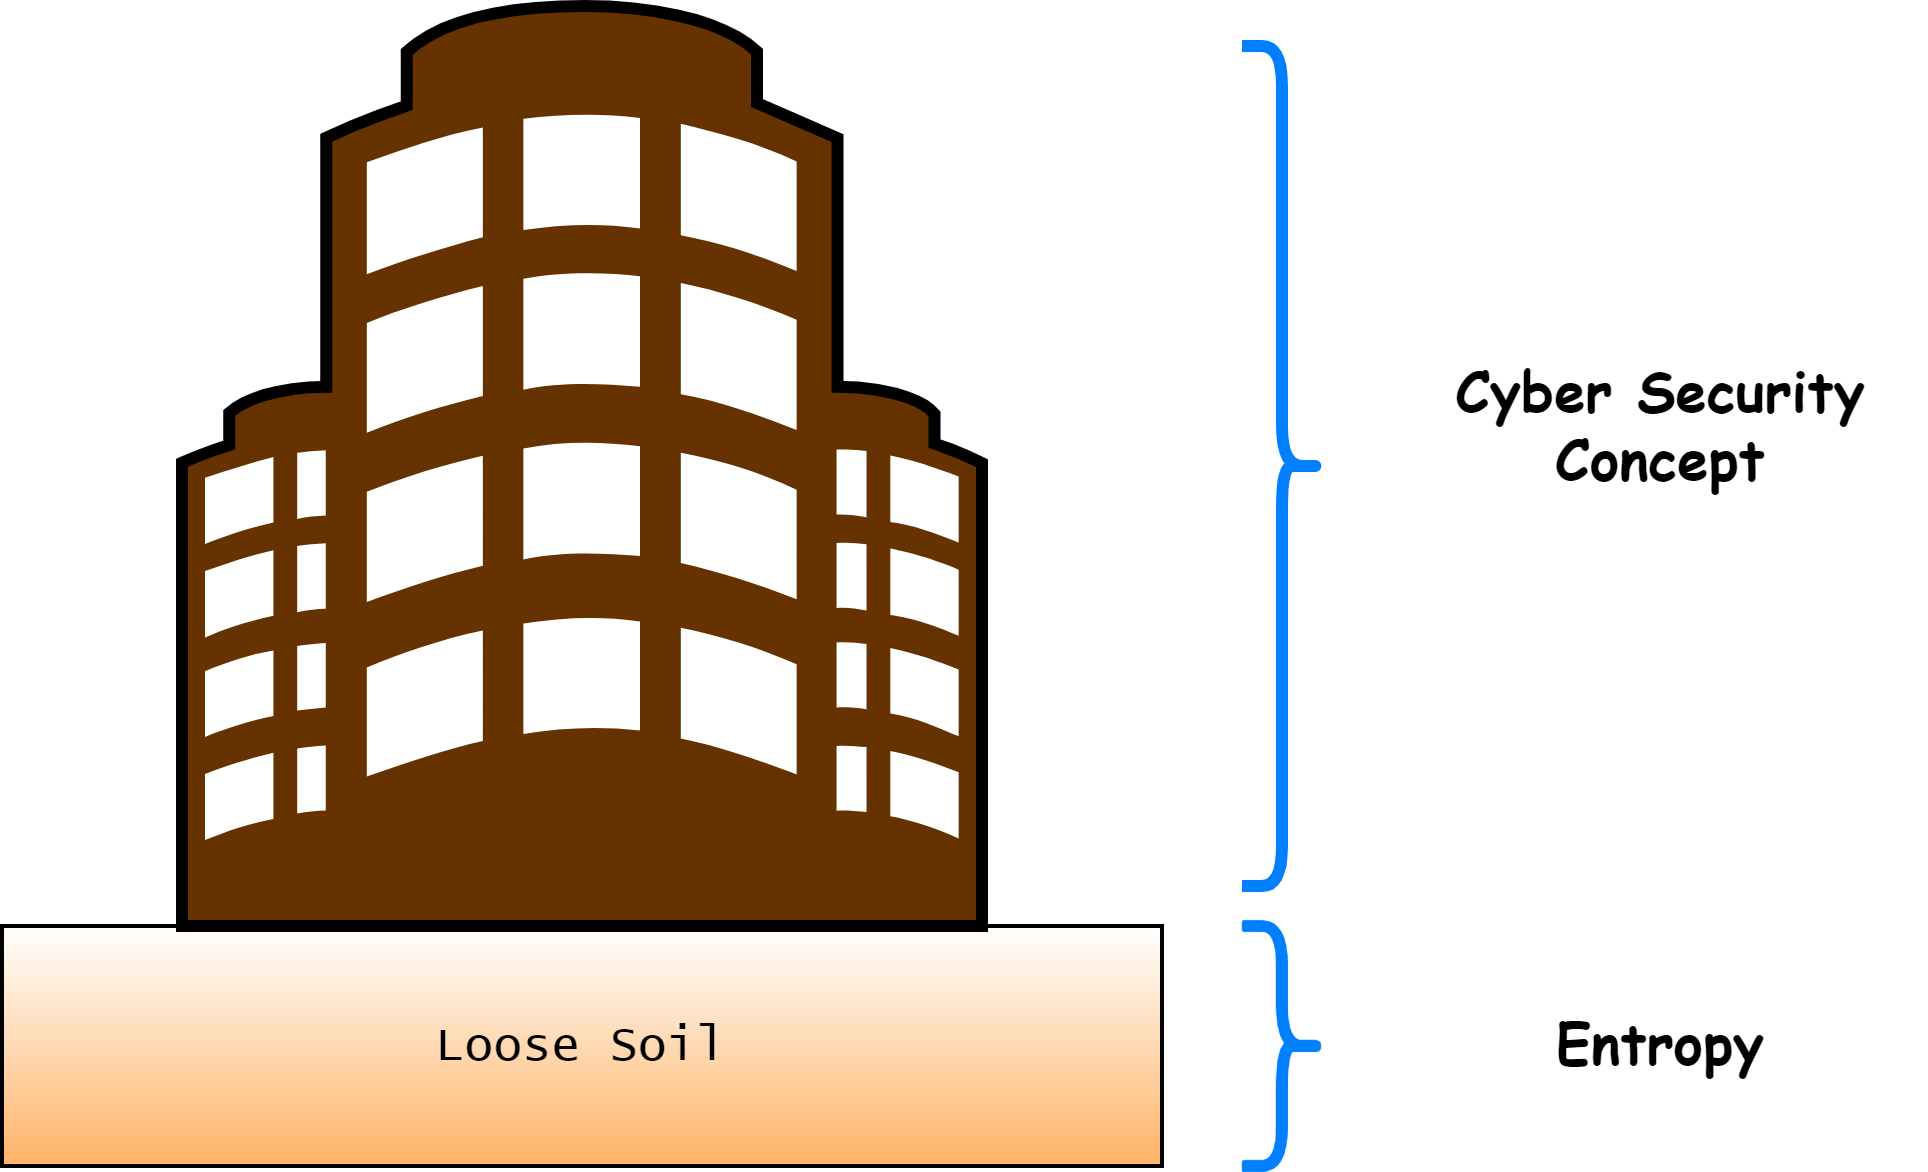
\includegraphics[width=0.75\textwidth]{gfx/diagrams/EffectOfWeakEntropy}
	\caption{Illustration of dependency of security concept on entropy}
	\label{fig:1:1}
\end{figure}







\chapter{Fundamentals}
\label{ch:fundamentals}

In this study we will be concentrating on the random numbers and generation of random numbers. Hence, we need to understand some of the basic components and terminologies before we get deeper into the topic.

%
% Section: Entropy
%
\section{Entropy}
\label{sec:fundamentals:entropy}

As we have seen in the Chapter \ref{ch:intro}, measure of the randomness is known as entropy. We will try to understand the entropy in detail.

To understand the entropy in an intuitive way, let us consider a random variable $X$. Now we will try to define entropy in terms of $X$.

\begin{enumerate}
	\item If consider $X$ in terms of bits, the amount of randomness in $X$ can be understood as entropy.
	\item In other terms, to save a draw from $X$ with compression, average amount of bits required is known as entropy.
	\item Average amount of Yes/No question required to be answered to guess the number $X$ can be defined as entropy.
\end{enumerate}

Considering above mentioned intuitive definitions, entropy can be represented as average amount of Information content in X. 

\begin{equation}
\label{eq:2:1}
H(X) = \sum_{x \in range(X)}  avg(I_{X}(x))
\end{equation}

Where, $X$ is a message or random variable, $I_{X}(x)$ is the information content in $X$ and $H(X)$ is the entropy of variable $X$.

%
%Section: Entropy Types
%
\section{Types of Measurements of Entropy} 
\label{sec:fundamentals:types}

In an "ideal world," all the intuitive definitions provided in section \ref{sec:fundamentals:entropy} hold true. Nevertheless, in a biased environment where the distribution of event occurrence is not uniform. Entropy cannot just be thought of as an average measure of freshness or information content. As a result, there exist numerous entropy measurement options. It is preferable to employ the appropriate type of entropy depending on the application for which it is being considered.

%
% Sub-Section: Shannon Entropy
%
\subsection{Shannon Entropy}
\label{subsec:fundamentals:types:shannon}

Let's start with Shannon entropy as we have already examined entropy as an average of information content. In 1948, Claude Shannon used mathematics to define the information entropy as,
\begin{equation*}
H(X) = \sum_{x \in range(X)} P_{X}(x)*\log_{2}\frac{1}{P_{X}(x)} 
\end{equation*}
\begin{equation}\label{eq:2:2}
H(X) = {-}\sum_{x \in range(X)} P_{X}(x).\log_{2}P_{X}(x) 
\end{equation}

This expression is known as Shannon’s entropy. This gives the average unpredictability in the random number $X$.\\

\underline{Intuitive Illustration:}\\\\
Consider set $A = \{1,1,1,1\}$, $B = \{1,1,1,0,1\}$ and $C = \{1,0,1,0,1,0\}$,\\\\
Probability of picking 1 and 0 in all the sets are correspondingly:\\

$P_{A}(1) = 4/4 = 1,\ P_{A}(0) = 0/4 = 0$\\
 
$P_{B}(1) = 4/5 = 0.8,\ P_{B}(0) = 1/5 = 0.1$\\

$P_{C}(1) = 3/6 = 0.5,\ P_{C}(0) = 3/6 = 0.5$\\\\
Let's now think about the surprising aspect of choosing 1 and 0 in every set:\\
Given that we know set A includes all 1, choosing 1 from it is not at all surprising.\\
Selecting 1 in set B is less shocking because it has a larger probability of happening. Picking 0 in set B, though, is more unexpected.\\
Given that set C has a 0.5 probability of both 1 and 0, choosing 1 and 0 there is equally unexpected.\\\\
Considering the probabilities and the surprising factors for picking the values out of all the three sets, we can observe that surprise is inversely proportional to probability.
\begin{equation*}
Surprise \propto \frac{1}{Probability}
\end{equation*}\\\\
Surprise cannot be easily defined as 1/Probability. Given that set A has a probability of 1 yet given our prior understanding of the link between surprise and probability, the surprise of choosing number one in set A should be zero. So, if we apply the definition given above, surprise becomes 1.\\
Hence, we use logarithmic function and define surprise as,
\begin{equation*}
Surprise = \log\left(\frac{1}{Probability}\right)
\end{equation*}\\
As we can observe that, if the probability is one surprise will yield to 0 and is the probability is 0 surprise will be undefined as we are trying to find which is not present. Figure \ref{fig:2:1} illustrates the relation between surprise and probability.
\begin{figure}[htbp]
	\centering
	\includegraphics[width=0.5\textwidth]{gfx/diagrams/Surprise_Prob_graph}
	\caption{Graph of surprise as a function of probability}
	\label{fig:2:1}
\end{figure}\\
Now, since we are dealing with the information theory, dealt information is binary. Hence, it makes sense to use logarithmic function to the base of 2. 
\begin{equation}\label{eq:2:3}
Surprise = \log_{2}\left(\frac{1}{Probability}\right)
\end{equation}\\
Information content of an element $I(X)$, also known as surprisal or self-information of an element.\\
Therefore, above equation \ref{eq:2:3} can be represented as,
\begin{equation*}
I_{X}(x) = \log_{2}\left(\frac{1}{Probability}\right)
\end{equation*}\\
Further considering probability of an element as P(x), equation can be rewritten as,
\begin{equation}\label{eq:2:4}
I_{X}(x) = \log_{2}\left(\frac{1}{P_{X}(x)}\right)
\end{equation}\\
If we are considering the numerous trails, then the average amount of surprise depends on the value of the surprise and the probability of observing that particular value of surprise.\\
Hence, 
\begin{equation}\label{eq:2:5}
avg\left(I_{X}(x)\right) = P_{X}(x)*\log_{2}\left(\frac{1}{P_{X}(x)}\right)
\end{equation}\\
Now considering the formula for Entropy as discussed in equation \ref{eq:2:1} and replacing $avg\left(I_{X}(x)\right)$ from equation \ref{eq:2:5}, Entropy H(X) can be written as,\\
\begin{equation*}
H(X) = \sum_{x \in range(X)}  P_{X}(x)*\log_{2}\left(\frac{1}{P_{X}(x)}\right)
\end{equation*}\\
Considering the property of logarithm, $\log(\frac{a}{b})\ =\ \log(a)\ {-} \ \log(b)$,
\begin{equation*}
	H(X) = \sum_{x \in range(X)}  P_{X}(x)*\left(\log_{2}(1) {-} \log_{2}\left(P_{X}(x)\right)\right)
\end{equation*}
\begin{equation*}
	H(X) = \sum_{x \in range(X)}  P_{X}(x)*\left(0 {-} \log_{2}\left(P_{X}(x)\right)\right)
\end{equation*}
\begin{equation}\label{eq:2:6}
H(X) = {-}\sum_{x \in range(X)} P_{X}(x).\log_{2}P_{X}(x) 
\end{equation}\\
This is the formula for Shannon Entropy.\\
The average amount of entropy present in the bitstring is given by Shannon entropy. The average quantity of entropy may give an overestimate because we are discussing it in the context of cryptography. A system's security may be compromised because of this overestimation of potential problems.

%
% Sub-Section: Min-Entropy
%
\subsection{Min Entropy}
\label{subsec:fundamentals:types:min}
The efficiency of the tactic of assuming the output of the entropy source that is most likely to occur is measured by min entropy. The min-entropy of the random number $X$ from the events that created it is correlated with the likelihood that a random number is properly predicted on the first try. In other words, min-entropy measures the lowest amount of information in the random variable $X$ that might be used to forecast the chosen value.\\
As was demonstrated in section \ref{sec:fundamentals:entropy}, the likelihood of information content may be expressed as euqation \ref{eq:2:4}: 
\begin{equation*}
I_{X}(x) = \log_{2}\left(\frac{1}{P_{X}(x)}\right)
\end{equation*}\\
From the understanding of min-entropy $H_{\infty}(X)$ can be presented as,
\begin{equation*}
	H_{\infty}(X) = \min_{x \in range(X)} I_{X}(x)
\end{equation*}\\
Replacing the value for $I_{X}(x)$ in above equation,
\begin{equation*}
	H_{\infty}(X) = \min_{x \in range(X)} \log_{2}\left(\frac{1}{P_{X}(x)}\right)
\end{equation*}\\
Considering Property of logarithm,
\begin{equation}\label{eq:2:7}
H_{\infty}(X) = {-}\min_{x \in range(X)} \log_{2}\left(P_{X}(x)\right)
\end{equation}\\
This formula can also be presented in terms of max function as,
\begin{equation}\label{eq:2:8}
H_{\infty}(X) = {-}\log_{2}\left(\max_{x \in range(X)} P_{X}(x)\right)
\end{equation}

Using min-entropy for the estimations in cryptography makes perfect sense since it offers the bare minimum of information needed to forecast the random number. This offers complete defence against any unanticipated events that might jeopardize security.

%
% Sub-Section: Max-Entropy
%
\subsection{Max Entropy}
\label{subsec:fundamentals:types:max}
Max entropy is also a measure of randomness, with a distribution which maximizes the entropy. Entropy of random variable $X$ is maximum, when the distribution of the events while choosing the random variable $X$ is evenly distributed. Hence, Max entropy always comes with the uniform distribution, which is expressed by constrained max entropy distribution. 

%
% Section: Entropy Source
%
\section{Entropy Source}
\label{sec:fundamentals:entropysource}
As described in the section \ref{sec:fundamentals:entropy} entropy is a randomness source, that is very basic necessity for any deterministic random number generator. Freshness or randomness should be having some form and we need some source to obtain the entropy. Entropy in information theory is always represented in the form of bitstream. In this section we describe the model of source to obtain the entropy bits.

\begin{figure}[htbp]
	\centering
	\includegraphics[width=0.75\textwidth]{gfx/diagrams/Entropy_Source_Model}
	\caption{Entropy Source Model}
	\label{fig:2:2}
\end{figure}

Figure \ref{fig:2:2} describes the entropy source model. Entropy source is entirely dependent on any unexpected or unpredictable event which is happening in the system. Any such events generally produce analog signal, that is further digitized to get the bitstring. Digitized noise data fetched unexpected event is conditioned to reduce the biasing of the string and in parallel health test validates the digitized noise to be used as a justifiable entropy.

%
% Section: Noise Source
%
\section{Noise Source}
\label{sec:fundamentals:noisesource}
Noise source as seen from the Figure \ref{fig:2:2} is the root of the entropy source model. This component is the that is based on the unforeseeable process responsible for providing the uncertain bits out of Entropy source. Few such chancy process produce binary samples which can directly be used but, in most cases, there is a need for digitization process that converts the output samples to bits.
\begin{figure}[htbp]
	\centering
	\includegraphics[width=0.75\textwidth]{gfx/diagrams/variety_of_noise_sources}
	\caption{Variety of Noise Sources}
	\label{fig:2:3}
\end{figure}

There are multiple sources that can be used as a noise source. Figure \ref{fig:2:3} shows wide range of potential noise sources and corresponding availability in Automotive ECU. Noise sources in any system can be mainly classified as:
\begin{description}
	\item[Physical Sources] These sources are founded on natural phenomena that produce random data or based on the hardware build TRNG. Physical noise sources can be divided into several groups, such as:
	\begin{itemize}
		\item Thermal noise is produced by the erratically moving electrons in a semiconductor or conductor.
		\item Shot noise is produced when electrons arrive at random in a wire or semiconductor.
		\item Radioactive materials decay, which is what causes radioactive decay.
		\item Noise in the atmosphere is caused by changes in the atmosphere of the Earth.		
	\end{itemize}
	\begin{figure}[htbp]
		\centering
		\includegraphics[width=0.25\textwidth]{gfx/diagrams/Filtered_sensor_output}
		\caption{Filtered Sensor Output}
		\label{fig:2:4}
	\end{figure}

	While raw sensor readings are typically not readily available for collection of entropy in most ECUs, physical sources typically provide significant degrees of randomness or high entropy outputs. The APIs will be made available for the gathering of entropy after the sensor values have been filtered. Values outside of the filter will be largely steady because the outputs are filtered. This lowers the output's entropy bits. Figure \ref{fig:2:4} illustrates the output available from the sensor.
	\item[Non-Physical Sources] These sources rely on artificial mechanisms that provide random data. There are various categories into which non-physical noise sources can be divided, including:
	\begin{itemize}
		\item User input: This refers to any input produced by users, such as keystrokes, mouse movements, and other unpredictable inputs.
		\item All data that is transmitted through a network, such as packet arrival times and packet sizes, is referred to as network traffic.
		\item Disk access patterns: These are any unpredictable disk access operations, like read and write operations.
		\item Process execution times: This covers the amount of time it takes for a process to run, which can be affected by a few variables and is sometimes challenging to forecast.		
	\end{itemize}
\end{description}

Entropy is exclusively provided by the noise source, which is the only part of the entropy source model. The source's characteristics must be understood for it to be used for entropy collection, making this knowledge crucial. the following qualities become crucial:
\begin{description}
	\item[Entropy] The quantity of freshness values or bits delivered in the output sample by the source. This is how entropy is defined, and a higher entropy guarantees a high level of security for the system.
	\item[Sampling Rate] Event-based noise sources offer entropy as soon as an event occurs, but for time-based noise sources, it's critical to assess and understand the rate at which the source's output is changing. 
	\item[Sample Size] Each selected noise source will have an output that is a specific length. To collect entropy during each sampling period, we need to know the size of the output sample.
	\item[Statistical Distribution] Entropy should be statistically dispersed across the sample, which means that random values in the output should be concentrated to a small number of bits yet uniformly scattered across the output's length.
	\item[Independence] The output of the source shouldn't be dependent on any other sources, prior outputs, or any other factors that make the output deterministic. This is known as the "independency" of the source.
\end{description}

%
% Section: Entropy Rate
%
\section{Entropy Rate}
\label{sec:fundamentals:entropyrate}
As we've seen, entropy may be thought of as a property of a probability distribution, like the mean or variance. Entropy is a measure of the uncertainty of the probability distribution on a bitstring produced by an entropy source rather than referring to any characteristic. Whereas the rate at which the entropy source is supplying entropy is known as the entropy rate. It is calculated as the judged quantity of entropy produced by a bitstring output from the source, divided by the total number of bits in the bitstring.
As an illustration, imagine an entropy generator that generates n-bit strings with m bits of entropy in each one. Then entropy rate can be simply written as,
\begin{equation*}
Entropy Rate = \frac{m}{n}
\end{equation*}

%
% Section: Conditioning
%
\section{Conditioning}
\label{sec:fundamentals:conditioning}
As we have discussed in the properties of the noise sources in section \ref{sec:fundamentals:noisesource}, output should be uniformly distributed among entire length of bitstream of output. But most of the noise source provide an output which in which the entropy bits will be concentrated to only certain portion. Also, bitstring generated in many cases will be biased. Conditioning is used to modify the bitstring to be used for cryptographical applications by reducing the biasing and distributing the entropy bits uniformly. 

\begin{figure}[htbp]
	\centering
	\includegraphics[width=0.75\textwidth]{gfx/diagrams/Conditioning_bitstring}
	\caption{Conditioning the Bitstream}
	\label{fig:2:5}
\end{figure}
 
\begin{figure}[htbp]
	\centering
	\includegraphics[width=0.7\textwidth]{gfx/diagrams/1-conditioning}
	\caption{Conditioning Process}
	\label{fig:2:6}
\end{figure}

Conditioning will not increase the entropy of any bitstring. It will increase the entropy rate of the output by condensing the entropy bits to shorter bitstring to match the application required bit length. Conditioning function can be illustrated as a distillation process using Figure \ref{fig:2:6}.\\

Algorithms which are used for conditioning should not reduce the entropy of the input bitstring. Hence, to avoid any wrong usage of the conditioning function, it is divided as two parts.

\begin{description}
	\item[Vetted Conditioning] Conditioning function that is examined extensively and approved by NIST. Following table provides the list of the vetted conditioned functions.
	\begin{table}[htbp]
		\centering
		\label{table:2:1}
		\begin{tabular}{||c c c||} 
			 \hline
			Conditioning Function & Narrowest Internal Width $(n_{w})$ & Output Length
			$(n_{out})$
			 \\ [0.5ex] 
			\hline\hline
			HMAC & hash-function output size & hash-function output size \\
			CMAC & AES block size = 128 & AES block size = 128 \\
			CBC-MAC & AES block size = 128 & AES block size = 128 \\
			Hash Funnction & hash-function output size & hash-function output size \\
			Hash\_df & hash-function output size & hash-function output size \\
			Block\_Cipher\_df & AES key size & AES key size \\
			\hline
		\end{tabular}
		\caption{Vetted Conditioning Function}
	\end{table}
	\item[Non-vetted Conditionin] Conditioning function that is not verified or approved by NIST. Any keyed or unkeyed cryptographic algorithm can be used as a conditioning.
\end{description}

If the vetted conditioning function is used for increasing the entropy rate, final entropy of the output$(h_{out})$ can be calculated with by using the algorithm as mentioned in NIST SP800-90. C-code of the algorithm in mentioned below. With the $n_{in}$ being input bitlength, $n_{out}$ being output bitlength, $h_{in}$ being input entropy bits and $nw$ being the narrowest width of the conditioning function, final entropy bits can be seen in output.

\begin{lstlisting}
long double output_entropy(int nin, int nout, int nw, int hin)
{
	long double phigh = pow(2, -1*hin);
	long double plow = (1 - phigh)/(pow(2,( nin - 1)));
	int n = min(nout, nw);
	long double Psi = (pow(2,(nin - n)))*plow + phigh;
	long double U = (pow(2,(nin - n))) + sqrt(2*n*(pow(2,(nin - n)))*log(2));
	long double omega = U*plow;
	long double maximum = max(omega, Psi);
	long double output = -1*log2(maximum);
	return output;
}

\end{lstlisting}

From the above-mentioned algorithm, it can be derived that, conditioned function increases the entropy rate. Output of the conditioning is said to be full entropy if input entropy bits provided is at-least the amount of required output bits. 

%
% Section: Left-over Hash Lemma
%
\section{Left-over Hash Lemma}
\label{sec:fundamentals:LHL}
Though Left-over hash lemma is exactly a measure of randomness, since we are dealing with the cryptographic use case it is very important to understand the Leftover hash lemma and its impacts.

The famous $Leftover Hash Lemma$ (LHL) states that (almost) universal hash functions are good randomness extractors. Despite its numerous applications, LHL-based extractors suffer from the following two limitations:
\begin{description}
	\item[Large Entropy Loss] to extract $v$ bits from distribution $X$ of min-entropy $m$ which are $\epsilon$-close to uniform, one must set $v\le m{-}2\log(1/\epsilon)$, meaning that the entropy loss $L_{def}=m{-}v\ge2\log(1/\epsilon)$. For many applications, such entropy loss is too large. 
	\item[Large Seed Length] the seed length $n$ of (almost) universal hash function required by the LHL must be at least $n\ge \min(u{-}v,v+2\log(1/\epsilon)){-}O(1)$, where $u$ is the length of the source, and must grow with the number of extracted bits.
\end{description}

%
% Section: 2.8	Health Test
%
\section{Health Test}
\label{sec:fundamentals:HT}
Validation and entropy estimation of the noise sources is a pre-requisite for the usage of the noise source for entropy collection. But, during the collection of entropy, noise sources are prone to failures due to the fragile nature. Hence, it is very important to detect the deviations of the source from the expected behaviour. Health Tests aim to detection such failures as quickly as possible with a high degree of probability.

As discussed in section \ref{sec:fundamentals:noisesource}, noise source should provide unbiased, independent statistically distributed data. But, as discussed in section \ref{sec:fundamentals:conditioning}, most of the noise sources don’t provide such output since noise sources are affected by the external conditions such as temperature, humidity, or electric field. Health tests should be typically designed to detect such failures or deviations based on the expected output. Health tests should raise an alarm in case there is a large reduction in the outputs' entropy, noise source failures occur, or if there are hardware malfunctions, and implementations are flawed.

%
% Section: Health Test Types
%
\section{Health Test Types}
\label{sec:fundamentals:HTT}
In section \ref{sec:fundamentals:HTT} we discussed about health tests, there are three types of health tests depending on the time when it is performed.

%
% Sub-Section: Start-up Test
%
\subsection{Start-up Test}
\label{subsec:fundamentals:HTT:SUT}
Start-up health checks are intended to be run after turning on, or rebooting, and prior to using the entropy source for the first time. Prior to being employed in normal operating conditions, they offer some assurance that the entropy source components are functioning as intended and that nothing has broken since the start-up tests were last performed. The samples taken from the noise source during the start-up tests must not be utilized for routine operations until the tests are finished; however, if there are no problems, the data may be used after the tests are over.

%
% Sub-Section: Continuous Test
%
\subsection{Continuous Test}
\label{subsec:fundamentals:HTT:CT}
Continuous tests concentrate on the behaviour of the noise source and seek to identify faults as the noise source generates outputs. Continuous checks are used to enable the entropy source to identify various faults in the underlying noise source. These tests must have a very low likelihood of triggering a false alarm during the normal operation of the noise source because they are run continuously on all digitized samples obtained from the noise source. Even throughout the course of a very lengthy service life, it is frequently exceedingly unusual in many systems that a fully operating device to report a failure.

There are two recommended tests, that are approved. When these tests are included as a part of continuous test, no other tests are needed. However, it is recommended that the developer add more continuous health tests that are specific to the noise source. Two tests are Repetition Count Test and Adaptive Proportion test.
\begin{description}
	\item[Repetition Count Test] The aim of the Repetition test is to detect immediately when catastrophic failures occur, that cause noise source to generate same output value for longer time. Repetition Count test is depicted in the Figure \ref{fig:2:7}. 
	\begin{figure}[h]
		\centering
		\includegraphics[width=0.5\textwidth]{gfx/diagrams/Repetition_Test}
		\caption{Repetition Count Test}
		\label{fig:2:7}
	\end{figure}
	\item[Adaptive Proportion Test] The Adaptive Proportion Test is made to identify a significant loss of entropy that could happen due to a physical malfunction or shift in the noise source's environment. To determine whether a sample value happens too frequently, the test continuously measures the local frequency of occurrence of the sample value within a sequence of noise source samples. Given the source's estimated entropy per sample, the test can therefore identify when a value starts to appear much more frequently than anticipated. Figure \ref{fig:2:8}S  illustrates the Adaptive Proportion test.
	\begin{figure}[htbp]
		\centering
		\includegraphics[width=0.4\textwidth]{gfx/diagrams/Adaptive_Prop}
		\caption{Repetition Count Test}
		\label{fig:2:8}
	\end{figure}
\end{description}

%
% Sub-Section: OD Test
%
\subsection{On-demand Test}
\label{subsec:fundamentals:HTT:ODT}
On-demand tests are source specific tests. These tests can be called any time. It is not mandatory to call these tests during the normal operation. However, source should be capable of performing on-demand tests of the output. On-demand tests can be called during boot. If start-up test is executed immediately after on-demand test collected outputs will not be available until start-up test is completed.  

%
% Section: Entropy Pool
%
\section{Entropy Pool}
\label{sec:fundamentals:entropypool}
Entropy is gathered in the form of a bitstream, as was evident from the previous sections. The system anticipates a higher level of entropy to remain secure. Yet, most of the entropy sources are unable to supply a whole bitstring at once. Concatenating the various outputs of the entropy source allows for the creation of bitstrings with increased entropy. The entropy pool is the name given to the memory space used to store the outputs from the entropy source.

When the system demands entropy at any given moment while it is operating and the collection of entropy upon request takes a long time to generate the required amount of entropy, the use of an entropy pool becomes crucial. The image below can be used to symbolize an entropy pool. The collecting of the data into the entropy pool is shown in Figure \ref{fig:2:9}.
\begin{figure}[htbp]
	\centering
	\includegraphics[width=0.75\textwidth]{gfx/diagrams/Entropy_Pool}
	\caption{Data collection into the Entropy pool}
	\label{fig:2:9}
\end{figure}

%
% Section: Security Strength
%
\section{Security Strength}
\label{sec:fundamentals:SS}
We must know the idea of security strength and how it relates to entropy now that we are aware of entropy and how it is accumulated. The degree of defense that a cryptographic method offers against attacks is referred to as security strength. It is frequently assessed in terms of how many operations must be performed to surpass the algorithm. The harder it is to defeat the algorithm and compromise the system, the higher the security strength. 

Another way to describe security strength is as a characteristic of cryptographic algorithms like DRBG that makes it difficult for an attacker to anticipate the outcome. As entropy is already understood to be the fundamental building block for the DRBG, we can state that security strength is directly connected with it. It is possible to express security strength as $security strength=\log_{2}(2^{entropy})$, which implies that security strength is equivalent to entropy, when output length of DRBG is less than the security strength.

%
% Section: DRBG
%
\section{DRBG}
\label{sec:fundamentals:drbg}
The Deterministic Random Number/Bit Generator, as mentioned in section \ref{sec:intro:Generation of Random Numbers}, is a random number generator that produces numbers using a deterministic algorithm. Figure \ref{fig:2:10} depicts the construction of a random number generator. As shown in the picture, the creation of random numbers solely depends on working/internal status if no further input, which is optional, is provided. 
\begin{figure}[htbp]
	\centering
	\includegraphics[width=0.75\textwidth]{gfx/diagrams/DRBG_Mechanism}
	\caption{DRBG Mechanism}
	\label{fig:2:10}
\end{figure}

Updates to and administration of the internal state are essential. Initial state acts as a foundation for the security strength of the generated random number because it is the input to the method, which is in a working condition. The seed is the starting point for the DRBG and is provided by the consuming application that needs a random integer. During setup and re-seeding, consuming applications update the working state.

Understanding the initial setup and reseeding procedures is crucial since they provide the primary strength of the generated random number. The DRBG is initially created at boot. Re-seeding is carried out according to seedlife. Re-seeding offers resilience to predictions and backtracking. This means that an adversary cannot forecast the numbers that will be generated in the future or go back and review the numbers generated in the past based on knowledge of the current functioning state.

The flow diagram in Figure \ref{fig:2:11}, can be used to illustrate how DRBG is instantiated. The security strength provided by the deterministic method utilized in DRBG is the highest security strength that can be produced by DRBG. Because of this, it is recommended that DRBG not be instantiated with a higher security strength and that the consuming application supply the entropy necessary to meet the security strength requirements.  Figure \ref{fig:2:12} shows the formation of initial internal state during the instantiation of the DRBG.
\begin{figure}[htbp]
	\centering
	\includegraphics[width=0.5\textwidth]{gfx/diagrams/Instantiation}
	\caption{DRBG instantiation}
	\label{fig:2:11}
\end{figure}

\begin{figure}[htbp]
	\centering
	\includegraphics[width=0.5\textwidth]{gfx/diagrams/Instantiation_Seed}
	\caption{Internal state formation during initialization}
	\label{fig:2:12}
\end{figure}

Re-seeding is a crucial component of the DRBG that offers prediction and resistance to backtracking, as was previously explained. Re-seeding provides newness to the internal state, making it harder for the enemy to predict the following random number. Re-seeding is done when prediction resistance is needed and the re-seed interval has passed, signalling that the security strength of the produced number has decreased. Figure \ref{fig:2:13} illustrates how to reseed the DRBG.
\begin{figure}[htbp]
	\centering
	\includegraphics[width=0.4\textwidth]{gfx/diagrams/Reseed}
	\caption{DRBG Re-seed mechanism}
	\label{fig:2:13}
\end{figure}
\begin{figure}[htbp]
	\centering
	\includegraphics[width=0.5\textwidth]{gfx/diagrams/Reseed_Seed}
	\caption{Working state formation during re-seed}
	\label{fig:2:14}
\end{figure}

Now that we've spoken about the instantiation and reseeding of the DGBG, it's time to understand how random numbers are generated. The primary function of the DRBG is to generate random numbers. When necessary, a random number generator can be summoned. The number will be created if the prediction resistance is not necessary or if the reseed interval has not yet been achieved after instantiation. The desired length of a random number must be supplied as an input during the creation process, and if further security is needed, additional input can also be supplied. Figure \ref{fig:2:15} illustrates the random number generation process of DRBG.

\begin{figure}[htbp]
	\centering
	\includegraphics[width=0.7\textwidth]{gfx/diagrams/DRBG_Generation}
	\caption{Random Number Generation process of DRBG}
	\label{fig:2:15}
\end{figure}

%
% Section: Hash based DRBG
%
\section{Hash based DRBG}
\label{sec:fundamentals:Hash_based_DRBG}
We spoke about generic DRBG in the previous section. We will talk about a specific DRBG function as an illustration of a cryptographically safe DRBG in this section. Three CSPRNGs are recommended by a series NIST SP800-90A, as shown in Table  \ref{table:2:2}. One of the three DRBGs that is often employed is hash-based. 
\begin{table}[htbp]
	\centering
	\begin{tabular}{||c c||} 
		\hline
		DRBG & Base algorithm used
		\\ [0.5ex] 
		\hline\hline
		Hash\_based\_DRBG & Hash\_df\\
		HMAC\_DRBG & HMAC\\
		CTR\_DRBG & Block ciphers such as AES\\
		\hline
	\end{tabular}
	\caption{Recommended DRBGs}
	\label{table:2:2}
\end{table}

The underlying basis technique for creating random numbers in hash-based DRBG employs a hash derivation function. Figure \ref{fig:2:16} shows the hash derivation function's operational flow.
\begin{figure}[htbp]
	\centering
	\includegraphics[width=0.5\textwidth]{gfx/diagrams/Hash_df}
	\caption{Hash Derivation Function}
	\label{fig:2:16}
\end{figure}

Hash\_based DRBG instantiation and reseeding are identical to generic DRBG, but an extra step is added to create a constant that will be utilized to create the internal state during the subsequent iterations of the generation process. The instantiation of Hash\_based DRBG is shown in Figure \ref{fig:2:17}, and its reseeding is shown in Figure 2.18.
\begin{figure}[htbp]
	\centering
	\includegraphics[width=0.45\textwidth]{gfx/diagrams/Instantiating_hash_drbg}
	\caption{Instantiation in Hash\_based DRBG}
	\label{fig:2:17}
\end{figure}
\begin{figure}[htbp]
	\centering
	\includegraphics[width=0.45\textwidth]{gfx/diagrams/reseeding_hash_drbg}
	\caption{Reseeding Hash\_based DRBG}
	\label{fig:2:18}
\end{figure}

In hash\_based DRBG, random integers are created as shown in Figure \ref{fig:2:19}. Hash\_gen, a function used in the generation process, is comparable to Hash\_df. Figure \ref{fig:2:20} provides an illustration of this function.
\begin{figure}[htbp]
	\centering
	\includegraphics[width=1.1\textwidth]{gfx/diagrams/Hash_based_DRBG_Generation}
	\caption{Generation of random numbers in Hash\_based DRBG}
	\label{fig:2:19}
\end{figure}
\begin{figure}[htbp]
	\centering
	\includegraphics[width=0.5\textwidth]{gfx/diagrams/Hash_gen}
	\caption{Hash\_gen Algorithm}
	\label{fig:2:20}
\end{figure}
\chapter{State of Art}
\label{ch:SoA}

In this Chapter we will understanding the current State of Art for random number generation. Initially we learn about the recommendations provided by NIST standard, then consider the entropy pooling algorithms such as Fortuna and Linux RNG.

%
% Section: NIST SP 800-90 Standard
%
\section{NIST SP 800-90 Standard}
\label{sec:SoA:NIST}

The NIST SP 800-90 series advises using one of three distinct methods for random number generation. RBG1, RBG2, and RBG3 are these designs. Each of these RBG constructions makes use of an entropy source as explained in section \ref{sec:fundamentals:entropy} and a DRBG as per table \ref{table:2:2}. The characteristics of RBG1, RBG2, and RBG3 are as shown in Table \ref{table:3:1}.

\begin{table}[htbp]
	\centering
	\label{table:3:1}
	\begin{tabular}{||p{2cm} p{2cm} p{2cm} p{2.5cm} p{2.5cm}||}
		\hline
		Design & Internal Entropy Source & Prediction Resistance & Full Entropy & Entropy Source Type
		\\ [0.3ex] 
		\hline\hline
		RBG1 & No & No & No & Physical \\
		RBG2 & Yes & Yes & No & Physical or Non-Physical\\
		RBG3 & Yes & Yes & Yes & Physical \\
		\hline
	\end{tabular}
	\caption{RBG Properties}
\end{table}

RBG1 does not offer prediction resistance, according to the interpretation of the table. In other words, RBG1 does not permit reseeding, which means that RBG1 is not given access to entropy sources after it has been created. Only once throughout the RBG's lifespan does RBG1 supply entropy to DRBG.

One or more entropy sources are built into the RBG2 architecture and used internally during the startup and reseeding of the DRBG. Reseeding enables the provision of prediction resistance in RBG2 construction.

RBG3 delivers output with a security level according to the length of random numbers that was requested. RBG3 generates a random number with complete entropy, in other words. There are two different versions of this architecture, which also resists predictions.

\begin{itemize}
	\item An RBG3(XOR) structure uses the exclusive-or (XOR) operation to combine the output of one or more certified entropy sources with the output of an instantiated, authorized DRBG.
	\item An RBG3(RS) architecture constantly reseeds the DRBG using randomness input from one or more certified entropy sources.
\end{itemize}

%
% Sub-Section: RBG1 Construction 
%
\subsection{RBG1 Construction}
\label{subsec:SoA:RBG1}
As discussed in section \ref{sec:SoA:NIST}, An RBG1 structure gives a device without an internal randomness source a supply of cryptographic random bits. Its security solely hinges on being safely instantiated from an RBG with access to an external physical entropy source.

Before being used for the first time by an RBG2 building or an RBG3 construction using a secure channel, an RBG1 construction is only instantiated (or seeded) once. After DRBG instantiation, there is no longer a randomness source accessible, hence an RBG1 construction cannot be reseeded and cannot consequently offer prediction resistance.

Subordinate DRBGs can be employed within the RBG1 security boundary since there is only a single chance for entropy to accumulate in RBG1 during its lifespan. RBG1 construction must be used to instantiate Sub-DRBGs. The use of one or more sub-DRBGs may be helpful for flash memory implementations when there are limitations on the number of write operations to the memory or when it is essential to use many DRBG instantiations for different purposes.
\begin{figure}[htbp]
	\centering
	\includegraphics[width=1\textwidth]{gfx/diagrams/RBG1_instantiation}
	\caption{RBG1 Construction}
	\label{fig:3:1}
\end{figure}
\begin{figure}[htbp]
	\centering
	\includegraphics[width=0.7\textwidth]{gfx/diagrams/Sub-DRBG}
	\caption{RBG1 Construction with Sub-DRBGs}
	\label{fig:3:2}
\end{figure}

Figure \ref{fig:3:1} illustrates the instantiation of RBG1 using RBG2 or RBG3 as a randomness source. \ref{fig:3:2} shows the instantiation of Sub-DRBGs in the security scope of RBG1.

%
% Sub-Section: Entropy Calculation Methods 
%
\subsection{Entropy Calculation Methods}
\label{subsec:SoA:ECM}
We talked about the building of RBG1 in the preceding part. We have not spoken about entropy calculation techniques since RBG1 accesses entropy through RBG2 or RBG3. As further discussions include the concept of entropy calculation, it is important to comprehend how entropy is calculated. There are two ways to get the entropy from the source, according to the NIST SP800-90 series. 
\begin{description}
	\item[Method 1] With this technique, a bitstring is created from one or more physical and non-physical sources. But for the entropy count, only physical sources will be employed.
	
	\underline{Illustration:}\\
	Assume that $P_{1},P_{2},\cdots,P_{x}$  are the equivalent bitstrings with $EP_{1},EP_{2},$ $\cdots,EP_{x}$  of entropy from the physical sources. The same holds good for non-physical sources $NP_{1},NP_{2},\cdots,NP_{x}$ and $ENP_{1},ENP_{2},\cdots,ENP_{x}$. Then, by concatenating outputs, the final bitstring for instantiation or reseeding are created.
	\begin{equation*}
	Bitstring = P_{1}||NP_{1}||NP_{2}||P_{2}||\cdots||P_{x}||NP_{x}
	\end{equation*}
	
	But the total entropy of the bitstring will only consider the entropy from physical sources such as,
	\begin{equation*}
	E_{total} = EP_{1} + EP_{2} + \cdots + EP_{x} 
	\end{equation*}
	\item[Method 2] This is method is like method 1, but here entropy from non-physical sources is also considered for the calculation of the overall entropy of the final bitstring.
	
	\underline{Illustration:}\\
	We will consider the same scenario as in method 1 with  $P_{1},P_{2},\cdots,P_{x}$ as outputs from physical sources with $EP_{1},EP_{2},\cdots,EP_{x}$  as corresponding entropy in the bitstring. $NP_{1},NP_{2},\cdots,NP_{x}$ as bitstring from non-physical sources with  $ENP_{1},ENP_{2},\cdots,ENP_{x}$ as respective entropy. Final bitstring is formed as,
	\begin{equation*}
	Bitstring = P_{1}||NP_{1}||NP_{2}||P_{2}||\cdots||P_{x}||NP_{x}
	\end{equation*}\\
	And the overall entropy of the final bitstring is
	\begin{equation*}
	E_{total} = EP_{1} + ENP_{1} + EP_{2} + ENP_{2} + \cdots +  EP_{x} + ENP_{x}
	\end{equation*}
\end{description}

%
% Sub-Section: RBG2 Construction 
%
\subsection{RBG2 Construction}
\label{subsec:SoA:RBG2}
On contrary to RBG1, RBG2 has access to the validated entropy source directly within its security boundary. Entropy source is used to gather the entropy required during instantiation or reseeding of the DRBG. An optional personalisation string or additional input required for the DRBG as discussed in section \ref{sec:fundamentals:drbg} can be included in the same boundary or can be obtained from outside the boundary. Figure \ref{fig:3:3} shows the construction of the RBG2.
\begin{figure}[htbp]
	\centering
	\includegraphics[width=0.7\textwidth]{gfx/diagrams/RBG2_Construction}
	\caption{RBG2 Construction}
	\label{fig:3:3}
\end{figure}
RBG2 can be constructed using one or more physical or non-physical sources. Based on the methods used for the consideration of the entropy RBG2 can also be classified as two variants RBG2(P) and RBG2(NP).
\begin{description}
	\item[RBG2(P)] creates a bitstring using one or more physical sources and, optionally, one or more non-physical sources. To calculate entropy, however, this version employs method 1. This implies that only entropy created by verified physical sources is considered for calculating the amount of entropy needed for instantiation or reseeding, as explained in section \ref{subsec:SoA:ECM}.
	\item[RBG2(NP)] employs any verified non-physical sources or physical source. This variation counts the required entropy using method 2. As a result, both physical and non-physical sources are given equal weight. Although both sources are equally important, it is advised to employ the conditioned outputs from non-physical sources since they are thought to not produce full-entropy output.
\end{description}

The same procedures as in section \ref{sec:fundamentals:drbg} are used for instantiation, reseeding, and the generation of random numbers from the DRBG in RBG2. However, the quantity of entropy that must be gathered from the source is the main factor to be considered in RBG2. To achieve the needed security strength, additional 128 bits of entropy must be given to the DRBG during instantiation if the RBG2 utilizes CTR\_DRBG (without derivation function). For instance, if s is the required security strength, the sources must provide $s+128$ bits of entropy. $3s/2$ bits of entropy must be gathered and sent to the DRBG during instantiation if any other suggested DRBG is utilized in the build.
\begin{figure}[htbp]
	\centering
	\includegraphics[width=0.7\textwidth]{gfx/diagrams/RBG2_Prediction_Resistance}
	\caption{RBG2 Prediction Resistance Mechanism}
	\label{fig:3:4}
\end{figure}

Prediction resistance in RBG2 is optionally supported. Even if the prediction resistance is supported by the RBG, usage of it is optional during the generation.  If the prediction resistance is requested during the generation and if it is supported by RBG, then the DRBG is reseeded during the generation process. Figure 3.4 illustrates the usage of prediction resistance in RBG2.

%
% Sub-Section: RBG3 Construction 
%
\subsection{RBG3 Construction}
\label{subsec:SoA:RBG3}
The RBG3 construction is made in a way to give the random numbers with full entropy. Given that RBG3 outputs full-entropy random numbers, entropy sources employed in the construction are anticipated to be validated physical sources that also produce full entropy. In contrast to RBG2, this construction solely uses Method 1 to calculate entropy.  RBG3 is always instantiated with the specified 256-bit security strength. As previously stated, RBG3 expects physical sources to provide full-entropy outputs. In any unforeseen circumstances, if a source fails to provide full-entropy and it goes undetected, the construction will continue to operate normally as RBG2, but if the source failure is discovered, the RBG will be terminated.

Entropy sources are a component of the RBG3 security boundary, and RBG3 continuously accesses them to obtain the necessary entropy. It is possible to create an implementation so that consuming applications can directly access the DRBG implementation that is utilized in an RBG3 construction. When complete entropy bits or a greater security level than what RBG1 and RBG2 constructions can offer are needed, an RBG3 construction might be beneficial.

According to the method used to produce the random numbers with full\-entropy, as was explained in section \ref{sec:SoA:NIST}, there are two possible ways to create RBG3.

%
% Subsub-Section: RBG3(XOR) Construction 
%
\subsubsection{RBG3(XOR) Construction}
\label{subsubsec:SoA:RBG3:XOR}
A DRBG and one or more certified entropy sources are both present in an RBG3(XOR) design. Full-entropy output is created by XORing the outputs of entropy sources and the DRBG. The output of the entropy sources must be converted to a full-entropy bitstring before being XORed with the output of the DRBG if the entropy sources are unable to deliver full-entropy output. Figure \ref{fig:3:5} describes the construction of RBG3(XOR).
\begin{figure}[htbp]
	\centering
	\includegraphics[width=0.7\textwidth]{gfx/diagrams/RBG3_XOR_Construction}
	\caption{RBG3(XOR) Construction}
	\label{fig:3:5}
\end{figure}

The DRBG is instantiated and reseeded in RBG3(XOR) similarly to RBG2, with the slight exception that the DRBG's intended strength is always 256. Entropy requirements from the RBG3 construction are identical to those from the RBG2 with $s+128$ for CTR\_DRBG (without differential function) and any other DRBG $3s/2$.

Generation processes of random numbers includes the collection of entropy and XORing with the output of the DRBG to provide full-entropy final output. Figure \ref{fig:3:6} illustrates the generation process of RBG3(XOR).
\begin{figure}[htbp]
	\centering
	\includegraphics[width=0.7\textwidth]{gfx/diagrams/RBG3_XOR_Gen}
	\caption{RBG3(XOR) Generation Process}
	\label{fig:3:6}
\end{figure}

%
% Subsub-Section: RBG3(RS) Construction 
%
\subsubsection{RBG3(RS) Construction}
\label{subsubsec:SoA:RBG3:RS}
The second RBG3 construction is RBG3(RS), where RS stands for Reseeding. This process continuously reseed the DRBG and generate the required amount bits with full security strength iteratively. Figure \ref{fig:3:7} provides the insight of RBG3(RS) construction.
\begin{figure}[htbp]
	\centering
	\includegraphics[width=0.7\textwidth]{gfx/diagrams/RBG3_RS_Construction}
	\caption{RBG3(RS) Construction}
	\label{fig:3:7}
\end{figure}

The instantiation, reseeding, and entropy requirements are identical to those of RBG3(XOR). But reseeding mechanisms are also a part of the generation process. The generation of random numbers using the RBG3(RS) structure is shown in Figure \ref{fig:3:8}. During the generating process, 128 bits of extra entropy bits must be given if the DRBG utilized is CTR\_DRBG (with or without differential function). On the other hand, 64 bits of extra entropy must be given for hash\_based DRBG.
\begin{figure}[htbp]
	\centering
	\includegraphics[width=0.6\textwidth]{gfx/diagrams/RBG2_Prediction_Resistance}
	\caption{RBG3(RS) Generation Process}
	\label{fig:3:8}
\end{figure}

%
% Section: Yarrow Algorithm
%
\section{Yarrow Algorithm}
\label{sec:SoA:YA}
Yarrow is a cryptographically safe pseudo-random number generator devised by John Kelsey, Bruce Schneier, and Niels Ferguson and published in 1999. A crucial design principle that makes Yarrow applicable to systems with a range of design constraints is the more-or-less independent nature of its components. The Yarrow's objective is to maximize the usage of the system's existing primitives to increase security. As a result, the design of Yarrow completely relies on block ciphers and one-way hash functions.
\begin{figure}[htbp]
	\centering
	\includegraphics[width=1\textwidth]{gfx/diagrams/Yarrow_Design_Principle}
	\caption{Yarrow Design Principle}
	\label{fig:3:9}
\end{figure}

Basic design principle of Yarrow is demonstrated in the Figure \ref{fig:3:9}. The Yarrow design concept is a combination four major steps. 
\begin{description}
	\item[Entropy Accumulation] In Yarrow, entropy accumulation is divided into two phases: collection of entropy from the source and pooling. The entropy is gathered from a variety of sources. Estimating the entropy is the step's most crucial factor to consider. Prior to use, the source is estimated, and samples are categorized according to sources while gathering entropy. Each source's contribution to entropy is then computed independently.
	 
	The fast pool and slow pool are the two pools that Yarrow employs. Each pool is a hash context, and each source has its own fast and slow pools. Samples from the source are kept in different pools in cycles. Fast pool offers frequent key reseeds so that new entropy may be added to the key more quickly. In contrast, a slow pool offers a higher but rarer quantity of entropy. 
	
	\item[Generation of Pseudo Random Numbers] Figure \ref{fig:3:10} serves as an illustration of the generation process. A n-bit counter, where n is the length of the block cipher output, serves as the generation process. After each generation cycle, C is increased, and the previous C is encrypted using Key k. It is seeded repeatedly using either a fast pool or a slow pool because, if the key were hacked at any time, it shouldn't leak too many old values or offer too many new values.
	\begin{figure}[htbp]
		\centering
		\includegraphics[width=1\textwidth]{gfx/diagrams/Yarrow_PRNG}
		\caption{Generation of Yarrow based Random Number}
		\label{fig:3:10}
	\end{figure}

	\item[Reseed Mechanism] To make it more difficult for an attacker to guess the block cipher's key, reseed is used to refresh the key. The pseudocode following demonstrates the reseed technique.
	
	\item[Reseed Control] This process regulates the reseed mechanism's interval. When a highly secure random number is required, reseeding is either explicitly carried out by the user application or implicitly carried out when the pool hits the threshold entropy level. The fast pool threshold in Yarrow-160 is 100 bits by a single source, and the slow pool threshold is 160 bits. To accomplish reseeding in a slow pool, two sources should meet this requirement.
	
\end{description}

%
% Section: Fortuna Algorithm
%
\section{Fortuna Algorithm}
\label{sec:SoA:FA}
The Fortuna algorithm was developed by John Kelsey, Bruce Schneier, and Niels Ferguson and is based on the enhancements made to the Yarrow algorithm. The fundamental concept of Fortuna is comparable to that of Yarrow and consists of pseudo-random number generation, reseeding, and entropy accumulation with pooling. However, the main issues with the Yarrow technique were the absence of entropy during startup time and knowing how much entropy to gather before utilizing it to reseed the PRNG. By gathering entropy at random from diverse sources, Fortuna attempts to alleviate these issues by dividing the entropy equally across 32 entropy pools in a round-robin method and employing a seed-file process. The Fortuna algorithm's core process flow is shown in Figure \ref{fig:3:11}.
\begin{figure}[htbp]
	\centering
	\includegraphics[width=0.5\textwidth]{gfx/diagrams/Fortuna_Design_Principle}
	\caption{Fortuna Design Principle}
	\label{fig:3:11}
\end{figure}

We will try to formulate the Fortuna algorithm in the same way as the Yarrow algorithm with an additional step describing the seed-file management.

\begin{description}
	\item[Entropy Accumulation] One of the primary distinctions between the Fortuna and Yarrow when compared to each other is entropy accumulation and pooling. As previously mentioned, one of the main issues with Yarrow is determining how much entropy to gather before use. The entropy is accumulated by Fortuna in 32 pools, $P_{0}\cdots P_{31}$, in a uniform and cyclical manner, correspondingly, using random data from various sources. Fortuna permits the use of 256 entropy sources that may be dynamically or statically labelled. Theoretically, all the pools should have unbound lengths to handle all the random events from outside sources. This causes significant memory limitations, which may be resolved by using a hash context in each pool. Figure \ref{fig:3:12} will describe the pooling mechanism.
	\begin{figure}[htbp]
		\centering
		\includegraphics[width=0.5\textwidth]{gfx/diagrams/Fortuna_Pooling_Concept}
		\caption{Pooling Mechanism in Fortuna}
		\label{fig:3:12}
	\end{figure}

	\item[Reseed Mechanism] How the freshness value is added to the key used in the generation process is determined by the reseed method. The reseeding technique is demonstrated in Figure \ref{fig:3:13}. A 32-bit counter is used as part of the reseed method to choose which pool should be considered. If $2^{i}$ divides the counter value without any remainder, the pool $P_{i}$ will be included in the reseed. As a result, higher numbered pools contribute to reseedings less frequently, but they do accumulate more entropy in between reseedings.
	\begin{figure}[htbp]
		\centering
		\includegraphics[width=0.5\textwidth]{gfx/diagrams/Fortuna_Reseed_Mechanism}
		\caption{Reseed Mechanism in Fortuna}
		\label{fig:3:13}
	\end{figure}

	\item[Reseed Control] This procedure establishes the necessary timing for reseeding. When "enough" random data has been added to the pools, only then can the generator be reseeded from them. To determine how much data is necessary to declare that "enough" random data has been collected, an optimistic estimate must be made. Additionally, it is advisable to keep the reseed rate to 10 reseeds per second to ensure that all pools are accumulating a sufficient level of entropy before reseeding.
	
	\item[Generation of Pseudo Random Number] Figure \ref{fig:3:14} shows the random number generation method and is identical to Yarrow's description. It comprises of a 128-bit counter and a 256-bit key for block cipher encryption of the counter value. As a block cipher, the generating procedure most frequently employs AES-256. To prevent the key value from being predicted, an additional two blocks of random numbers are created throughout each generation process and utilized as a key for the following iteration.
	\begin{figure}[htbp]
		\centering
		\includegraphics[width=1\textwidth]{gfx/diagrams/Fortuna_PRNG}
		\caption{Generation of Fortuna based Random Number}
		\label{fig:3:14}
	\end{figure}

	\item[Seed-file Management] When Fortuna is first started, a "seed file" gives the generator a seed. This initial seed enables the generator to generate random data even before the accumulator has accumulated sufficient entropy. A fresh seed is instantly created and written to the seed file when the seed file is read at start-up. This information is utilized to produce a higher-quality seed as Fortuna builds up entropy. It is advised that a fresh seed file be created every 10 minutes, although this greatly depends on the application and the rate at which entropy is building up.
\end{description}

%
% Section: Linux RNG
%
\section{Linux RNG}
\label{sec:SoA:LRNG}
The initial implementation of the Linux-RNG(LRNG) was provided by Theodore Ts'o in 1994. LRNG is one of the most widely used CSPRNG. The Linux-RNG is a random number generator that uses hardware events detected by the Linux kernel as noise sources to feed a deterministic random number generator. The architecture of LRNG is shown in Figure \ref{fig:3:15}. 
\begin{figure}[htbp]
	\centering
	\includegraphics[width=1\textwidth]{gfx/diagrams/LRNG_Arch}
	\caption{Linux RNG Architecture}
	\label{fig:3:15}
\end{figure}

LRNG architecture or design flow can be explained using following parts: 

\begin{description}
	\item[Aggregation of random data into pools] Entropy sources in LRNG may be thought of as events that the Linux kernel detects, as was explained above. Entropy pool, also known as input pool in the context of LRNG, is a Blake2s message digest. Any new event will be added to the input pool with the Blake2s update. 
	
	Pool updating is a little more complicated in situations when there are interrupt-based events. Fast pool is a basic memory structure to which interrupt-based events are added. Fast pool is being managed as a SipHash 1-0 / HalfSipHash utilizing an empty key. One fast pool is present in each CPU core. When the count reaches 64 or if it has been more than one second since the last merge, entropy from the fast pool is merged into the input pool. The Aggregation of the Random Data into the Pools is shown in Figure \ref{fig:3:16}.
	\begin{figure}[htbp]
		\centering
		\includegraphics[width=1\textwidth]{gfx/diagrams/LRNG_Pooling}
		\caption{Aggregation of the random data into the input pool in LRNG}
		\label{fig:3:16}
	\end{figure}

	Aggregation of random data into pools can be characterized as follows. After the occurrence of a hardware event, such as an interrupt, the event is awarded an entropy estimation by the Linux-RNG. The event time and the event value are hashed into the entropy pool, the Blake2s state.
	
	\item[Generation of the Random Numbers] LRNG uses chacha20 DRNG for the generation of the random number. Bases on timing difference between request and generation, requests can be classified based on:
	\begin{itemize}
		\item Unrestricted generation of random numbers, which means that random data is created whether the ChaCha20 DRNG or the entropy pool has received enough entropy.
		\item With blocked generation, random numbers are only produced when the original entropy obtained by the entropy pool or the ChaCha20 DRNG was at least 256 bits. When the 256-entropy bit barrier is achieved, calls to blocked generation behave similarly to unrestricted calls.
	\end{itemize}
	
	The LRNG's random number generation method may be divided into two steps as shown in Figure \ref{fig:3:17} and \ref{fig:3:18}.  
	\begin{figure}[htbp]
		\centering
		\includegraphics[width=1\textwidth]{gfx/diagrams/LRNG_EE}
		\caption{Extraction and Expansion Mechanism}
		\label{fig:3:17}
	\end{figure}

	\begin{figure}[htbp]
		\centering
		\includegraphics[width=1\textwidth]{gfx/diagrams/LRNG_Gen}
		\caption{ChaCha20 DRNG Operation}
		\label{fig:3:18}
	\end{figure}

	\begin{description}
		\item[Extract and Expand Mechanism] The concatenated output from the input pool and the output of 256 bits from an optionally installed CPU-based random number generator, such as Intel's RDSEED, are used to create a new key during the extract phase. The Blake2s hash context is reset using the resultant message digest to collect the further data from the noise sources. The output of the extract phase is also utilized in the expand phase, which creates random bits with a 32-byte size that are used as the seed for the ChaCha20 DRNG key.
		
		\item[ChaCha20 DRNG] The ChaCha20 DRNG operates by invoking the ChaCha20 DRNG block operation repeatedly until the requested number of bytes are generated. Hence, the output function of this DRNG is based on the ChaCha20 block operation. the counter value of the state is incremented by one after each ChaCha20 block operation. To ensure backtracking resistance, the fast-key-erasure approach specified in is applied.
	\end{description}
	
\end{description}

Every generation checks the reseed status of the key; if it has been more than 60 seconds since the last reseed, the pool is used to reseed the key. Reseeding occurs every (n + n/2) seconds for the first two minutes following startup, where n is the number of seconds after the reboot.

%
% Section: Chapter Summary
%
\section{Chapter Summary}
\label{sec:SoA:Summary}
The state-of-the-art designs for entropy collection and random number generation have been covered in this chapter. Although the NIST SP 800-90 standard offers a foundation for any architecture, it is often not practicable. Practical solutions are offered by Yarrow and Fortuna for systems with reliable randomness sources. The most used CSPRNG in many embedded devices is Linux RNG. However, LRNG also anticipates sources to offer random numbers with a high rate of entropy. The practical drawbacks of SoA will be discussed in the following chapter, and a workable architecture for automotive ECUs will be designed.
\chapter{Ein weiteres Kapitel}
\label{ch:chapter03}

Acronym \acf{AES}. 

%
% Section: Listen
%
\section{Listen}
\label{sec:chapter03:listen}
citation \cite{RANDOM-1998}

\begin{itemize}
 \item Enumeration with bullets
 \item Cras cursus ligula et tellus viverra sit amet accumsan orci consequat. Mauris eget elit enim, in mollis justo. Mauris ornare condimentum varius. Praesent suscipit sagittis eros, at accumsan justo adipiscing vel.
 \item Etiam a orci tellus. Cum sociis natoque penatibus et magnis dis parturient montes, nascetur ridiculus mus. Nullam iaculis congue ligula eget lacinia. Proin dapibus elit eu odio egestas dapibus. Etiam nunc dolor, sagittis et volutpat quis, rhoncus a tortor.
\end{itemize}

Nunc non tortor nisl, sed fringilla est. Sed feugiat, est sed imperdiet aliquam, nisl elit lobortis nisl, sit amet ultrices metus eros vitae metus. Integer tincidunt, nisi id consectetur pharetra, nibh tortor tempus ipsum, id sollicitudin erat lacus at diam. Etiam aliquet venenatis aliquet.

\begin{enumerate}
 \item Enumeration with small numbers
 \item Nulla dapibus, ante ac sagittis molestie, neque nulla venenatis turpis, non scelerisque lorem sapien non turpis. Sed dolor magna, vestibulum imperdiet condimentum vel, imperdiet ac mi. Cras in orci egestas purus rhoncus congue. Cras cursus leo nec turpis laoreet non malesuada est pretium.
 \item Nunc ut tortor massa. Fusce ullamcorper mauris eget tellus egestas faucibus. Ut nec nunc quis lectus iaculis ultrices. Lorem ipsum dolor sit amet, consectetur adipiscing elit.
\end{enumerate}

Suspendisse dignissim tellus vitae ante ullamcorper luctus. Maecenas consectetur massa a massa vestibulum non egestas ipsum bibendum. Vestibulum porttitor, tortor at porttitor tristique, magna justo vestibulum sapien, a semper augue magna in orci. Mauris pretium laoreet nisi, sit amet ultricies sapien rutrum ut. Suspendisse placerat risus et magna accumsan. Ased fringilla est. Sed feugiat, est sed imperdiet aliquam, nisl elit lobortis nisl, sit amet ultrices metus eros vitae metus. Integer tincidunt, nisi id consectetur pharetra, nibh tortor tempus ipsum, id sollicitudin erat lacus at diam. Etiam aliquet venenatis aliquet. Mauris sit amet leo id ligula fringilla pharetra. In id neque metus, eu congue libero. Suspendisse egestas imperdiet nulla, in blandit dolor venenatis vel.

\begin{enumerate}
 \item Enumeration with small caps (alpha)
 \item Second item ed ac risus dolor, ac molestie tellus. Fusce nulla lacus, viverra vel tempus et, viverra eget augue. Nunc id dui sed velit feugiat tristique. Integer at velit justo, eget ornare nulla.
 \item Suspendisse cursus, nisl non pharetra dapibus, nunc ligula sollicitudin sem, in vehicula leo nunc et neque. Sed lacinia dapibus erat, eu dictum ligula auctor a. Phasellus ut mi sapien, in sodales turpis. Nunc pharetra varius metus eget convallis.
\end{enumerate}


\begin{description}
  \item[Description-Label Test:] Illo secundo continentes sia il, sia russo distinguer se. Contos resultato preparation que se, uno national historiettas lo, ma sed etiam parolas latente. Ma unic quales sia. Pan in patre altere summario, le pro latino resultato.
  \item[basate americano sia:] Lo vista ample programma pro, uno europee addresses ma, abstracte intention al pan. Nos duce infra publicava le. Es que historia encyclopedia, sed terra celos avantiate in. Su pro effortio appellate, o.
  \item[Cras venenatis:] Purus et posuere lacinia, nisl sapien dapibus metus, a ornare enim odio in ipsum. Quisque imperdiet nibh metus, in fringilla tellus. Duis varius dui eget orci commodo ac sollicitudin est placerat. Cras varius tincidunt arcu, quis imperdiet nibh rhoncus vel. Sed non justo orci, non accumsan felis. Maecenas condimentum convallis.
\end{description}

%
% Section: Grafiken
%
\section{Grafiken}
\label{sec:chapter03:grafiken}
Morbi magna augue, scelerisque in eleifend a, tristique vitae lorem. Vivamus non elementum nisi. Aliquam erat volutpat. Nunc pharetra, tortor ut adipiscing bibendum, orci ipsum mollis felis, ut euismod eros purus at tellus. Sed blandit eros at ante mattis in elementum tortor pharetra. Vivamus molestie mattis orci. Quisque ullamcorper, purus sit amet luctus viverra, turpis arcu imperdiet eros, sit amet viverra nisi ligula ut felis.

\subsection{Einfache Grafiken}
\label{sec:chapter03:grafiken:simple}
Vestibulum ante ipsum primis in faucibus orci luctus et ultrices posuere cubilia Curae; Donec sed ante odio. Integer semper, nibh id sollicitudin adipiscing, odio elit blandit mi, sit amet luctus mauris velit nec velit. Aenean commodo cursus magna, id mollis sapien gravida eu. Aenean eleifend, leo dignissim sodales mattis, tellus ante tempor nunc, vulputate tristique nisl metus sit amet tellus. Nullam sollicitudin, metus sit amet sagittis interdum, metus purus dapibus lacus, pharetra lobortis erat enim a leo. Suspendisse a augue in purus tempor blandit. Aliquam malesuada porttitor nibh vel adipiscing. In mi est, vulputate nec dapibus quis, pharetra vel lacus. Sed pellentesque egestas pretium. Praesent orci risus, ornare non accumsan id, gravida sed lectus. Mauris fermentum viverra neque at dignissim. Sed consectetur auctor lorem, eget volutpat urna sodales id. Etiam pellentesque velit quis sapien tempus convallis. 

\begin{figure}[htbp]
 \centering
 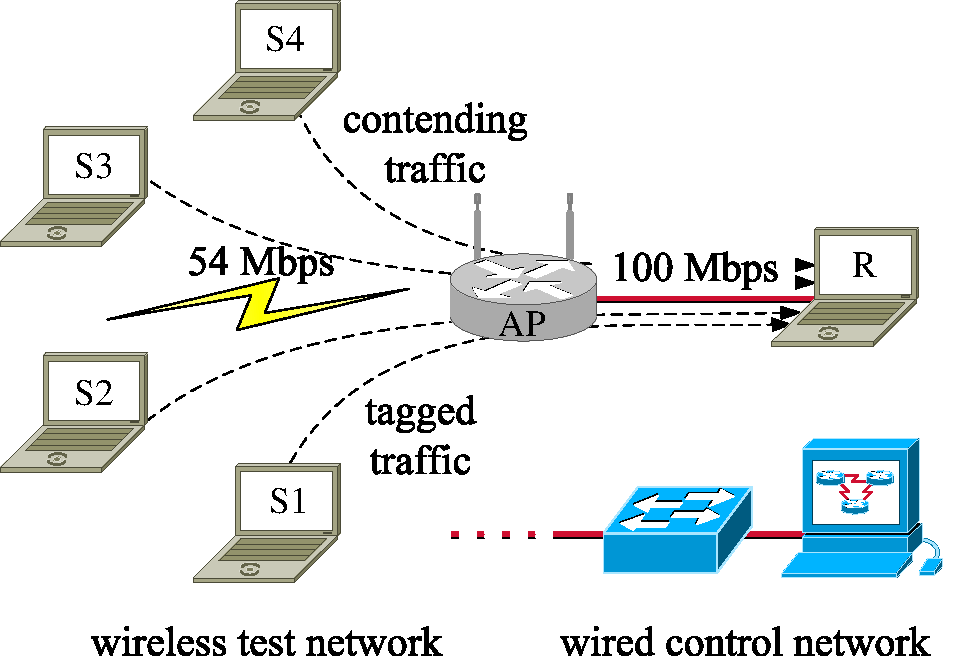
\includegraphics[width=0.5\textwidth]{gfx/examples/setup}
 \caption{Dies ist eine einfache Grafik}
 \label{fig:chapter03:setup}
\end{figure}

Aenean blandit neque eget nunc euismod ac dignissim enim euismod. Nullam semper, orci vitae elementum pretium, est lorem sodales justo, id lobortis nunc felis et justo. Cras tortor orci, rhoncus a commodo quis, aliquam eu dui. Donec pulvinar, arcu ornare consequat ultricies, purus dui accumsan massa, id auctor magna justo nec risus. Nulla bibendum, est nec ornare venenatis, lacus diam pretium augue, sed convallis orci sapien vitae lectus. In blandit massa aliquam felis feugiat fringilla.

\subsection{Grafiken mit Subfloat}
\label{sec:chapter03:grafiken:subfloat}
Quisque non massa neque. In at placerat lacus. Integer urna augue, laoreet ac mattis sed, posuere ut turpis. Nunc a metus quis elit placerat ultricies vel a eros. Quisque condimentum aliquet fermentum. Integer arcu est, suscipit quis lacinia at, volutpat nec tortor. Proin feugiat tristique est eget luctus. Suspendisse porta mauris sed sapien egestas sit amet volutpat tellus ultricies. Nulla vulputate semper turpis sed blandit. Phasellus at tortor pulvinar nisi luctus gravida.



\begin{figure}[h]
	
	\begin{subfigure}{0.5\textwidth}
		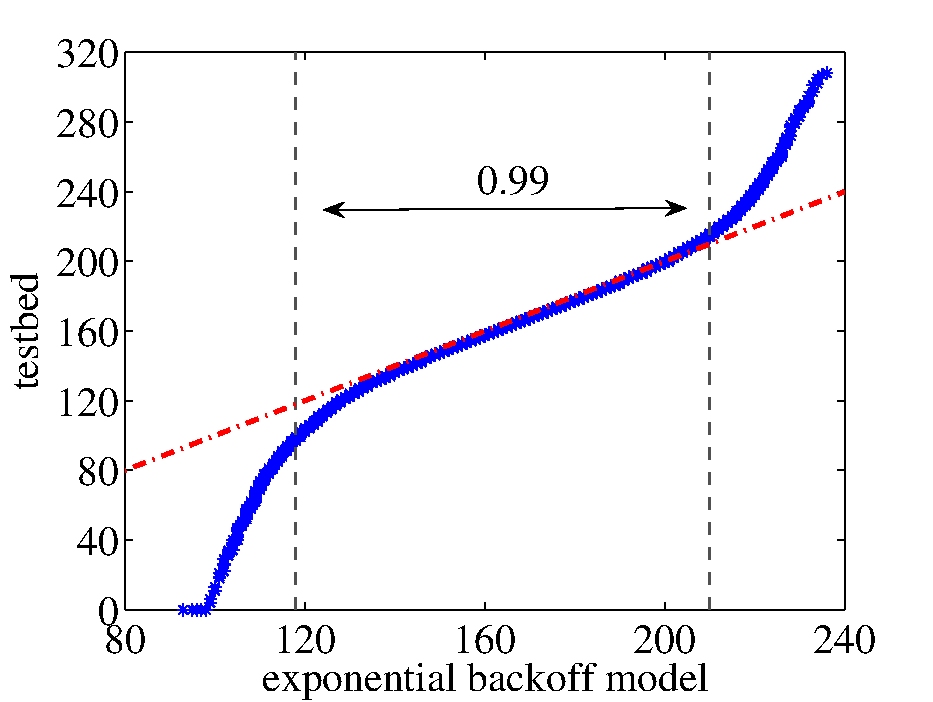
\includegraphics[width=0.9\linewidth, height=6cm]{gfx/examples/qq-plot_gaus_vs_160} 
		\caption{PTAT}
		\label{fig:a}
	\end{subfigure}
	\begin{subfigure}{0.5\textwidth}
		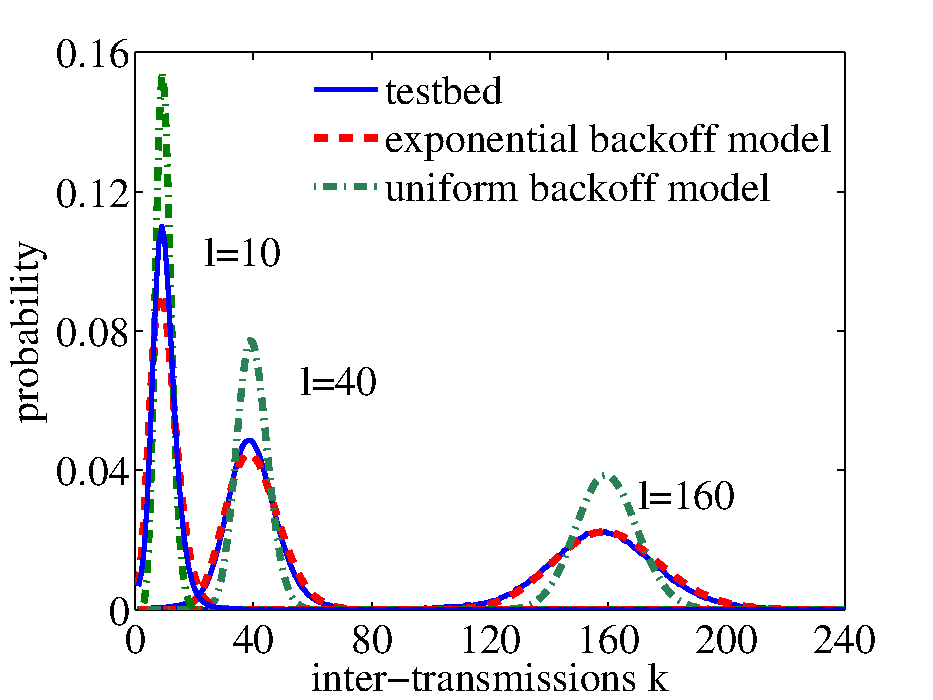
\includegraphics[width=0.9\linewidth, height=6cm]{gfx/examples/pdf_gaus_vs_uni_vs_10_40_160}
		\caption{CTAT}
		\label{fig:b}
	\end{subfigure}\\	
	\begin{subfigure}{0.5\textwidth}
		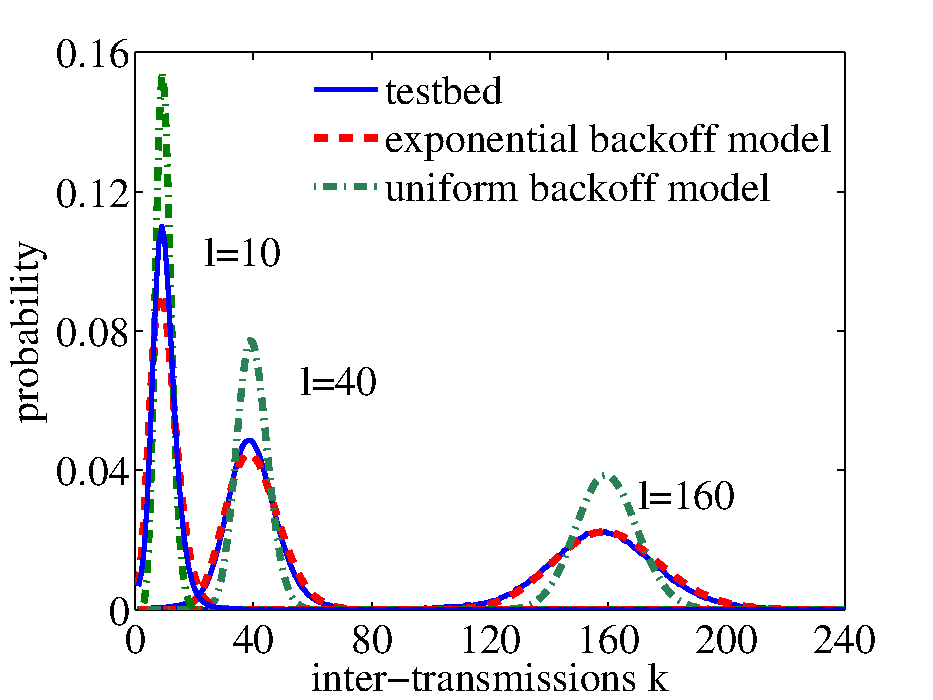
\includegraphics[width=0.9\linewidth, height=6cm]{gfx/examples/pdf_gaus_vs_uni_vs_10_40_160} 
		\caption{Counter1}
		\label{fig:c}
	\end{subfigure}
	\begin{subfigure}{0.5\textwidth}
		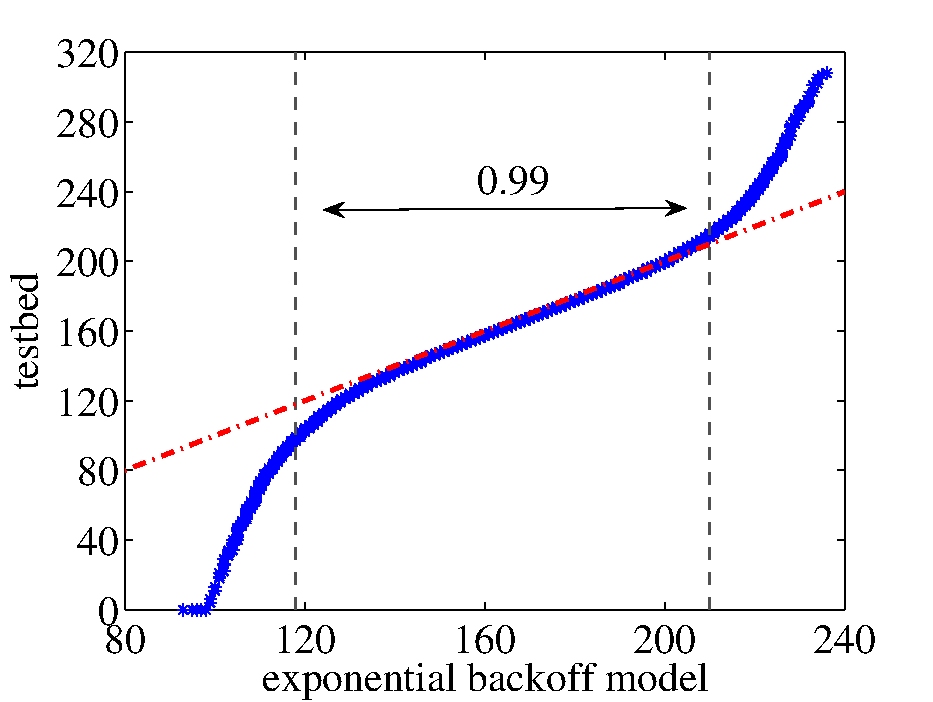
\includegraphics[width=0.9\linewidth, height=6cm]{gfx/examples/qq-plot_gaus_vs_160}
		\caption{Counter2}
		\label{fig:d}
	\end{subfigure}
	
	\caption{Example of sub-float diagram}
	\label{fig:6:2}
\end{figure} 


\subsection{Grafiken mit Minipage}
\label{sec:chapter03:grafiken:minipage}
Donec gravida consequat arcu, et mollis tortor posuere vitae. Sed pharetra turpis a ante commodo accumsan. Suspendisse leo nulla, accumsan sit amet dapibus in, posuere eget turpis. Vivamus enim sapien, porta id placerat eget, laoreet sed massa. Class aptent taciti sociosqu ad litora torquent per conubia nostra, per inceptos himenaeos.

\begin{figure}[htbp]
  \centering
  \begin{minipage}[b]{5 cm}
    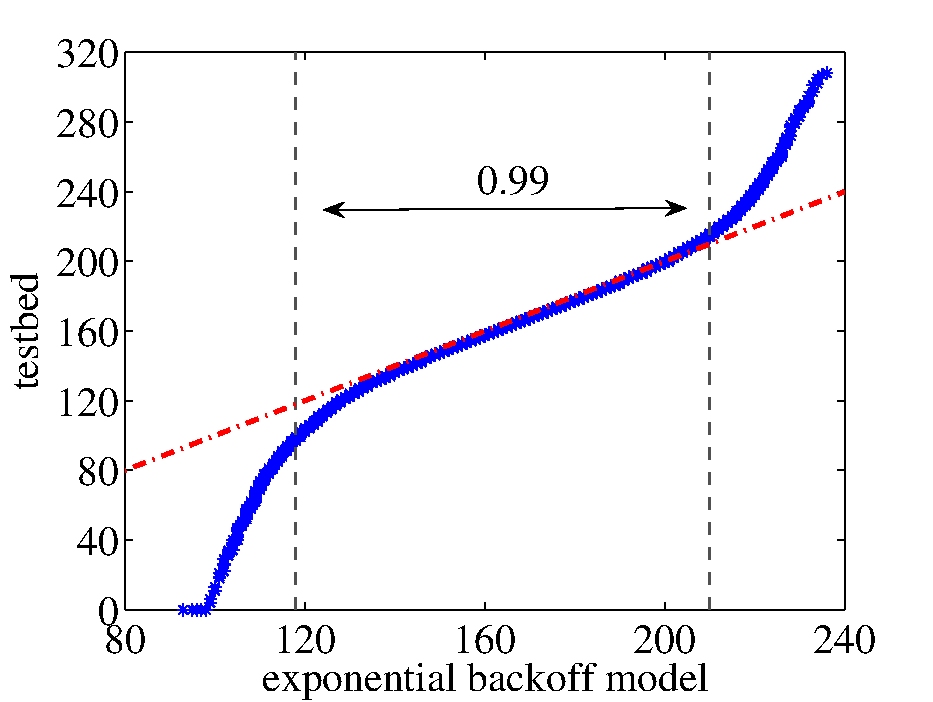
\includegraphics[width=\linewidth]{gfx/examples/qq-plot_gaus_vs_160} 
    \caption{Minipage-Grafik Nummero uno}
    \label{fig:chapter03:minipage:grafik1}
  \end{minipage}
  \begin{minipage}[b]{5 cm}
    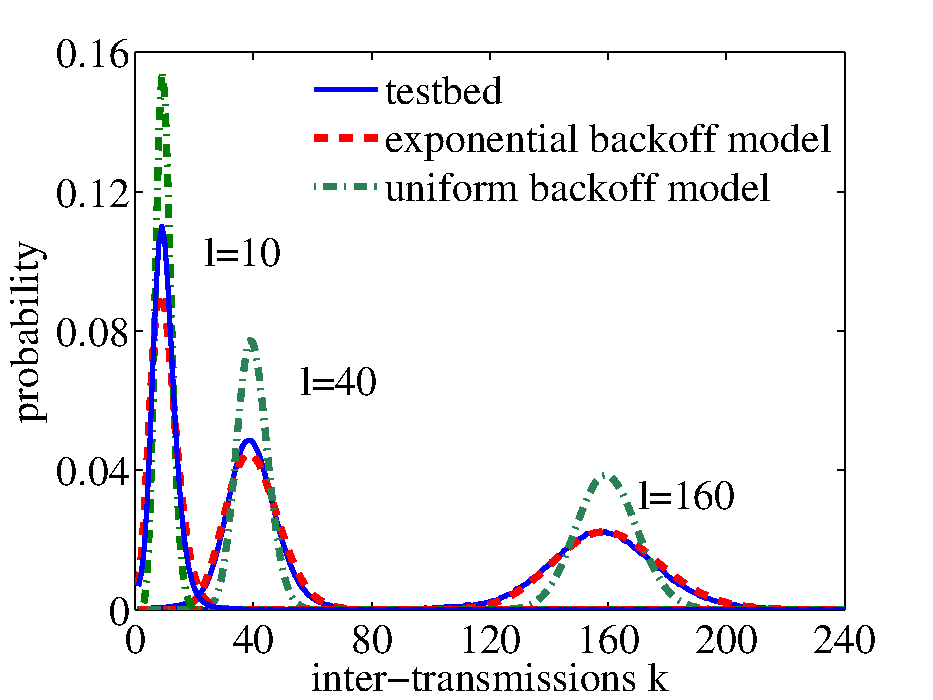
\includegraphics[width=\linewidth]{gfx/examples/pdf_gaus_vs_uni_vs_10_40_160}  
    \caption{Minipage-Grafik Nummer zwei}
    \label{fig:chapter03:minipage:grafik2}
  \end{minipage}
\end{figure}

In vitae est eget velit mattis lobortis. In hac habitasse platea dictumst. Quisque aliquam quam et justo pellentesque ullamcorper. Curabitur elementum mattis leo facilisis tincidunt. Fusce posuere viverra ultricies. Cras eget velit et ipsum gravida imperdiet et hendrerit orci.

Maecenas fringilla viverra urna ut egestas. Nulla sagittis molestie libero eget luctus. Nulla non odio sit amet magna vehicula tincidunt. Nulla accumsan ornare placerat. In posuere scelerisque quam, sed posuere urna eleifend quis. Pellentesque sed quam quis dui vulputate convallis ut ac diam. In hac habitasse platea dictumst. Donec molestie auctor dapibus. Vivamus in erat risus, ut aliquet diam. Duis vel velit ante, id ullamcorper turpis. Lorem ipsum dolor sit amet, consectetur adipiscing elit. In accumsan ornare tellus a porttitor. Etiam facilisis dui et sem eleifend id luctus nisl scelerisque. Aenean quis commodo libero. Nulla quis semper dolor. 

%
% Section: Tabellen 
%
\section{Tabellen}
\label{sec:chapter03:tabellen}
Sed lobortis vestibulum euismod. Vivamus vestibulum gravida nisi vitae condimentum. Nullam nec lacus nibh. Phasellus arcu magna, varius eget viverra a, elementum eu dolor. Aliquam erat volutpat. Sed nibh leo, vestibulum quis lacinia in, vestibulum sollicitudin nulla. In iaculis, purus in imperdiet sagittis, tortor diam pellentesque lectus, eget faucibus ante elit at tortor.

%
% Section: Listings 
%
\section{Listings}
\label{sec:chapter03:listings}
Aliquam ut pretium lectus. Curabitur in eros et sapien aliquet luctus ut sit amet eros. Proin et libero non mi venenatis aliquet at sed lorem. Ut sed enim mi, id viverra eros. Cras metus ante, placerat id commodo at, molestie non libero. Aenean eu risus erat, vel consequat metus. Sed malesuada metus sit amet nisl viverra hendrerit.


%
% Section: Equations
%
\section{Equations}
\label{sec:chapter03:equations}
Pellentesque sed quam quis dui vulputate convallis ut ac diam. In hac habitasse platea dictumst. Donec molestie auctor dapibus. Vivamus in erat risus, ut aliquet diam. Duis vel velit ante, id ullamcorper turpis.
%
\begin{equation}
 U = R * I
\end{equation}

Lorem ipsum dolor sit amet, consectetur adipiscing elit. In accumsan ornare tellus a porttitor. Etiam facilisis dui et sem eleifend id luctus nisl scelerisque. Aenean quis commodo libero. Nulla quis semper dolor.
%
\begin{equation}
 I = \frac{U}{R} 
\end{equation}

In the following we use probability theory to derive closed-form expressions for the fairness that is achieved among $M$ contending stations. We tag station $M$ and denote $K_i$ the inter-transmissions of station $i = 1 \dots M-1$ and let $K = \sum_{i=1}^{M-1} K_i$. The conditional probability $P[K\!=\!k|l]$ can be defined for $M \ge 2$ as
%
\begin{equation}
\mathsf{P}[K\!=\!k|l] = \mathsf{P} \Biggl[\sum_{i=1}^{M-1} K_i = k \Big| l \Biggr]
\label{eq:chapter03:exactpmf}
\end{equation}
%
where the random variables $K_i$ are the integers that satisfy
%
\begin{equation*}
\sum_{j=1}^{K_i} b_i(j) \le \sum_{j=1}^{l} b_M(j) \;\;\; \textmd{and} \;\;\; \sum_{j=1}^{K_i+1} b_i(j) > \sum_{j=1}^{l} b_M(j) .
\end{equation*}


%
% Section: Theorem and Proof
%
\section{Theorem and Proof}
\label{sec:chapter03:theorem}
We use the central limit theorem to derive the long-term fairness. In the sequel, we denote normal random variables $N(\mu,\sigma^2)$ where $\mu$ is the mean and $\sigma^2$ the variance.
%

%
%
For $M=2$ we have from (\ref{eq:chapter03:exactpmf}) that
%
\begin{equation*}
\mathsf{P}[K \!<\! k|l] = \mathsf{P} \Biggl[\, \sum_{j=1}^k b_1(j) > \sum_{j=1}^l b_2(j) \Biggr]
\end{equation*}
%
and after expansion and some normalization this equals
%
\begin{equation*}
= \mathsf{P}\Biggl[ \frac{\sum_{j=1}^{l}b_2(j) - l\mu}{\sigma\sqrt{l}} - \frac{\sum_{j=1}^{k}b_1(j) - k\mu}{\sigma\sqrt{l}} < \frac{\mu(k-l)}{\sigma\sqrt{l}} \Biggr].
\end{equation*}
%
Using the central limit theorem it follows that
%
\begin{equation*}
\mathsf{P}[K \!<\! k|l] \approx \mathsf{P} \biggl[ N(0,1) - N \biggl(0,\frac{k}{l}\biggr) < \frac{\mu(k-l)}{\sigma\sqrt{l}} \biggr] .
\end{equation*}
%
Since the normal distribution with zero mean is symmetric we can replace the subtraction of $N(0,k/l)$ by addition. Furthermore, the sum of two normal random variables $N(\mu_1, \sigma_1^2)$ and $N(\mu_2, \sigma_2^2)$ is normal with $N(\mu_1+\mu_2, \sigma_1^2+ \sigma_2^2)$ such that
%
\begin{equation*}
\mathsf{P}[K \!<\! k|l] \approx \mathsf{P} \biggl[ N\biggl(0,\frac{k+l}{l}\biggr) < \frac{\mu(k-l)}{\sigma\sqrt{l}} \biggr] .
\end{equation*}
%
Finally, we use that if $X$ is $N(a\mu,a^2\sigma^2)$ then $Y = X/a$ is $N(\mu,\sigma^2)$ with $a^2 = (k+l)/l$ to standardize the result.
%

Th. \ref{th:chapter03:twostationsgaussian} assumes i.i.d. random countdown values. It does, however, not make any assumption about their distribution.

\chapter{Implementation}
\label{ch:Imp}
As we have discussed the RNG architecture and framework design in chapter \ref{ch:CD}, we will discuss how the architecture and framework are implemented in this chapter. We will also discuss some integration hints to integrate the generated code into a project. As an example of integration, an ultrasonic ECU is considered (A project supported by the cybersecurity team at BEG).

%
% Section: Framework Description
%
\section{Framework Description}
\label{sec:Imp:FD}
As mentioned in section \ref{sec:CD:FD}, a UI-based code framework was considered in the design phase to be implemented for higher visual clarity. A Python-based UI was implemented, as Python provides ease of implementation and extendibility. Figure \ref{fig:5:1} explains the flow of the framework for code generation implemented. The framework consists of three parts:

\begin{description}
	\item[Framework Configuration] Configuration provides the flexibility to the framework to add or modify the source according to the project’s limitations. As the framework is Python based, the configuration file is also a Python file. Developers can access this file to add new sources or modify the source properties.
	
	\item[Properties Selection for RNG] The user performs the selection of properties. The user is provided with a provision for selecting noise sources, corresponding properties, RNG requirements, and system properties. This provision is made available using GUI. PyQT5 (Python QT UI designer) based UI designer tool is used to develop the GUI.
	
	\item[Code Template] The generation of code requires a template. Jinja2 code templates are used for this purpose. The code template holds the generic implementation of the architecture, as discussed in section \ref{subsec:CD:AD:AD}. Selected parameters from the GUI will be replaced in the template to generate the final integrative code.
\end{description}

\begin{figure}[!h]
	\centering
	\includegraphics[width=0.8\textwidth]{gfx/diagrams/implementation}
	\caption{Framework flow}
	\label{fig:5:1}
\end{figure}

The framework was designed and implemented with the following
principles in mind:
\begin{itemize}
	\item Ease of use: The user interface is designed to be intuitive and user-friendly. GUI is split into three screens to differentiate the properties to be selected and the operations to be performed.
	
	\item Flexibility: Framework is kept as flexible as possible to add new sources and modify the source properties based on the project evaluations. Code templates add more flexibility to use any number of sources with any selected property.
	
	\item Efficiency: The code generation tool is optimized to generate code quickly and accurately. Generated code from the template can be directly integrated into the complete software module.
\end{itemize}

The framework’s efficiency, adaptability, and simplicity are some of its advantages. It streamlines the process of writing code by offering a user-friendly interface and pre-made templates. However, the framework’s code generation engine could be constrained by the available templates, and customization choices might be limited for use cases with more intricate use cases. Additionally, engineers have to perform initial evaluations before selecting the properties.


%
% Section: Framework Implementation
%
\section{Framework Implementation}
\label{sec:Imp:FI}
As described in section \ref{sec:Imp:FD} framework consists of three parts. The configuration file holds pre-evaluated sources and corresponding properties that the developer can modify. The properties section is implemented based on UI design, and code templates are used to generate the c-code for random number generation in ECU. Three parts are explained in detail in this section. However, before explaining each part, we need to consider the prerequisites that should be performed in each project using the framework.\\
Prerequisites:
\begin{itemize}
	\item Identify potential noise sources and evaluate the properties of noise sources such as entropy estimate, sampling rate and sample size.
	
	\item Evaluation of security requirements of the project to decide on security strength, desired length of random numbers and reseed interval.
	
	\item Analysis of system criteria such as available crypto libraries such as bosch crypto-library (BCL) containing the bosch-specific implementation of cryptographic algorithms or common crypto-library (CCL) holding other secure algorithms. Memory and runtime limitations of the ECU are necessary as well.
\end{itemize}


%
% sub-section: Framework Configuration
%
\subsection{Framework Configuration}
\label{subsec:Imp:FI:FC}
As mentioned in section \ref{sec:Imp:FD}, the configuration is handled using a Python file holding all the initial information required. Configuration holds pre-evaluated noise sources and their properties, as shown in Figure \ref{fig:5:1}.

\begin{figure}[!h]
	\centering
	\includegraphics[width=1\textwidth]{gfx/diagrams/Config_File}
	\caption{Example of configuration of pre-evaluated noise sources}
	\label{fig:5:2}
\end{figure}

The configuration file also contains all the selectable properties to provide user-friendly access to developers while using GUI.
\begin{itemize}
	\item The list "Noise\_Sources" holds all the identified noise sources.
	
	\item The object source\_prop["source"]["EntropyPerBit"] holds the pre-estimated entropy rate per bit of the source.
	
	\item The object source\_prop["source"]["BitPerSample"] holds the size of the output sample.
	
	\item The object source\_prop["source"]["SampleRate"] holds the rate at which samples were collected for the estimation.
\end{itemize}
 The configuration will be made available to the developers to modify according to the project needs. Any newly identified sources can be added to list and create a new structure to hold the properties of the sources. 

%
% sub-section: Noise Source selection
%
\subsection{Properties Selection for RNG}
\label{subsec:Imp:FI:NSS}
Properties selection is the second step in generating code after loading the configuration into the GUI tool. Properties selection is vital, as this determines the strength of the random number to be generated. It is essential to evaluate the noise sources by the developer before parameters are selected. To avoid confusion for users, GUI is divided into three tabs.

The first tab contains the noise source selection checkboxes and a text display box. All the pre-evaluated noise sources will be listed in the tab for the selection. Text display will show the properties from of the selected noise sources the configuration file as described in previous section \ref{subsec:Imp:FI:FC} for the developer to know the properties to define other sampling rates and sample sizes. Figure \ref{fig:5:3} shows the first GUI tab.

\begin{figure}[!h]
	\centering
	\includegraphics[width=1\textwidth]{gfx/diagrams/gui_tab1}
	\caption{Source selection tab}
	\label{fig:5:3}
\end{figure}

Once the noise sources are selected, the second tab provides the provision to select the parameters to be considered for using each noise source based on properties displayed in the previous tab. In this tab, a developer can configure the rate at which the sample should be collected, the size in bytes and the continuous health tests. Additionally, provision is provided to enter a function pointer for the on-demand test. Figure \ref{fig:5:3} shows the properties update tab of GUI.

\begin{figure}[!h]
	\centering
	\includegraphics[width=1\textwidth]{gfx/diagrams/gui_tab2}
	\caption{Source properties update tab}
	\label{fig:5:4}
\end{figure}

Finally, the properties of the RNG are selected in the third tab. The developer can select if the RNG has to produce full-entropy random numbers. If the project requires full-entropy output, the 320 + 128 entropy bits are gathered from the sources that produce a random number of desired lengths. Else required, $3/2 * SS + 128$ bits of entropy are gathered to produce a random number of length 256 bits. Numbers $3/2*SS$ and 320 are suggested by the NIST recommendations \cite{SP90C-2022} considering the highest possible length of the random number being 256 bits. This length results from the DRBG algorithm being used, i.e., SHA-256; SHA-256 is a secure hash algorithm producing 256 bits of output. Users can also provide the if backtracking/prediction resistance is required to enable the automatic reseeding.

Since the tool is generated for the customer projects developed in Bosch, most projects use base software, including crypto libraries. Hence, the user can also select the library in the base software. As the initial version of the tool supports only hash-based DRBG with SHA-256 as a function, it is selected as a default. However, provision for an update of the tool to support other DRBG functions is provided. Figure \ref{fig:5:5} shows the RNG properties selection tab for non-full-entropy random numbers, and figure \ref{fig:5:6} for full-entropy output.

\begin{figure}[!h]
	\centering
	\begin{minipage}[b]{5 cm}
		\includegraphics[width=\linewidth]{gfx/diagrams/gui_tab3_1} 
		\caption{RNG properties selection tab for non-full-entropy random number}
		\label{fig:5:5}
	\end{minipage}
	\begin{minipage}[b]{5 cm}
		\includegraphics[width=\linewidth]{gfx/diagrams/gui_tab3_2}  
		\caption{RNG properties selection tab for full-entropy random number}
		\label{fig:5:6}
	\end{minipage}
\end{figure}

\begin{figure}[!h]
	\centering
	\begin{minipage}[b]{5 cm}
		\includegraphics[width=\linewidth]{gfx/diagrams/gui_tab3_3} 
		\caption{Time for gathering entropy bits for non-full-entropy random number}
		\label{fig:5:7}
	\end{minipage}
	\begin{minipage}[b]{5 cm}
		\includegraphics[width=\linewidth]{gfx/diagrams/gui_tab3_4}  
		\caption{time for gathering entropy bits for full-entropy random number}
		\label{fig:5:8}
	\end{minipage}
\end{figure}

Once all the properties are selected, a push button to calculate the best time required to gather the entropy is provided, and the time is displayed in the text edit widget. This calculation is based on the rate and size of the sample collected from all the selected sources and their respective entropy estimates. Users can modify the properties based on the results of calculated time and then generate the code by clicking the push button. Figure \ref{fig:5:7} and \ref{fig:5:8} show the calculated time for gathering entropy bits to produce non-full-entropy and full-entropy output, respectively.

%
% sub-section: Code structure
%
\subsection{Code Template}
\label{subsec:Imp:FI:CS}
The result of pressing the “Generate Code” push button is the generation of c-code implementing the architecture described in section \ref{subsec:CD:AD:AD}. Jinja2 package is used for writing the generic templates. As described in section {sec:CD:ACF}, parameters selected in the GUI will replace the templated part of the code.

Each selected noise source generates a context of the structure as defined in the listing below. APIs will be generated to fetch the samples from each source selected in GUI. API also contains the number of bytes to be fetched from the source. The number of bytes to be collected from each source during each call is calculated based on the schedule rate and entropy per bit of the source output. The flow diagram of the code for gathering the entropy into the pool is shown in figure \ref{fig:5:9}.

\begin{lstlisting}

	typedef struct esPropCtx
	{
		const float minEntropy;
		const uint8 numBitsPerSample;
		const uint8 reqNumOfBytes;
		uint8 entropyRequired[MAX_BYTES_FROM_SOURCE];
		boolean startUpTestSt;
		sint16 (*getNoise)(const struct esPropCtx *self, uint8 reqNumOfBytes, uint8* bytes);
		boolean (*startUpTest)(struct esPropCtx *self);
		contTest_t contHealth;
		boolean (*repetitionTest)(struct esPropCtx *self);
		boolean (*AdaptiveProportionTest)(struct esPropCtx *self);
		boolean (*onDemandTest)(struct esPropCtx *self);
	}esPropCtx_t;

\end{lstlisting}

\begin{figure}[!h]
	\centering
	\includegraphics[width=1\textwidth]{gfx/diagrams/flow_diagram_pooling}
	\caption{Code flow diagram for pooling entropy bits}
	\label{fig:5:9}
\end{figure}

Once the entropy pooling is done, reseeding of the DRBG has to be handled to provide the prediction resistance. Figure \ref{fig:5:10} illustrates the flow diagram for DRBG reseed mechanism.
\begin{figure}[!h]
	\centering
	\includegraphics[width=1\textwidth]{gfx/diagrams/flow_diagram_drbg}
	\caption{Code flow diagram for reseed mechanism}
	\label{fig:5:10}
\end{figure}

To summarize the implementation process, pre-evaluated properties of the noise sources are added to the configuration. This configuration is used for user selection of properties and scheduling the noise source. Once all the properties are selected, two files, “entropy.c” and “entropy.h”, are generated, containing the code for entropy gathering and pseudo-random number generation.

%
% sub-section: Integration
%
\subsection{Integration}
\label{subsec:Imp:FI:Int}
Lastly, files have to be integrated into the complete ECU software for the code to be executed in the ECU. To integrate the files following steps have to be considered.
\begin{enumerate}
	\item Files should be copied to the corresponding location in the software project and included in the makefile for build purposes.
	
	\item Call the \textit{void collectEntropy(void);} method in 10ms task, this method further schedules the noise source for fetching the output samples.
	
	\item API \textit{getXXXNoise} will be generated for each noise source with the number of bytes to be fetched. Update \textit{getXXXNoise} API to map the corresponding source API to gather noise. An example of \textit{getXXXNoise} is shown in figure \ref{fig:5:11}.
	\begin{figure}[!h]
		\centering
		\includegraphics[width=1\textwidth]{gfx/diagrams/api_example}
		\caption{Example API for getTimerNoise}
		\label{fig:5:11}
	\end{figure}	
	
	Noise source APIs are specific to each source and ECU. Therefore, generating the API \textit{getXXXNoise} mapped to the source's actual API is impossible. Here, provision for the mapping of the source is provided. Based on the number of bytes requested from the source, samples should be mapped to \textit{bytes} pointer, and if any error occurs during the collection, the return code has to be set to $-1$.
	
	\item Include the function declaration to link the pointer if any on-demand tests are requested.
	
	\item Use the API \textit{getRandomNumber(uint8* randNum, uint16 length);} to fetch the pseudo random number.
	
	\item Compile and run the executable in ECU.
	
\end{enumerate}


%
% Section: Chapter Summary
%
\section{Chapter Summary}
\label{sec:Imp:CS}
In this chapter, we discussed the implementation strategies to develop a GUI and template to generate the code based on the properties selected by the developer. We also discussed the integration hints to add the generated code to the project and compile it to execute in ECU. In the next chapter, we will discuss the results and perform the risk analysis of the target entropy.




\chapter{Results and Analysis}
\label{ch:RA}
In this chapter we will discuss about the results obtained from designed architecture in this master thesis. The collection of samples, sensors used to collected the entropy and theoretical analysis of the final entropy rate estimation are done in accordance with the objectives as outlined in chapter \

%
% Section: Evaluation of Acrhitecture
%
\section{Evaluation of Acrhitecture}
\label{sec:RA:EA}

%
% Section: Risk Analysis of Target Entropy
%
\section{Risk Analysis of Target Entropy}
\label{sec:RA:RATE}


\chapter{Conclusion}
\label{ch:end}

%
% Section: Possible Extensions
%
\section{Possible Extensions}
\label{sec:end:RA}

%
% Section: Mitigation Strategies
%
\section{Mitigation Strategies}
\label{sec:end:Summary}

\appendix
%************************************************
\chapter{Introduction to the ClassicThesis style}\label{ch:classicthesis}
%************************************************
The ClassicThesis bundle for \LaTeX\ has two goals:
\begin{enumerate}
    \item Provide students with an easy-to-use template for their
    Master's
    or PhD thesis. (Though it might also be used by other types of
    authors
    for reports, books, etc.)

\end{enumerate}
The bundle is configured to run with a \emph{full}
MiK\TeX\ or \TeX Live\footnote{See the file \texttt{LISTOFFILES} for
needed packages. Furthermore, \texttt{classicthesis}
works with most other distributions and, thus, with most systems
\LaTeX\ is available for.}
installation right away and, therefore, it uses only freely available
fonts. (Minion fans can easily adjust the style to their needs.)

People interested only in the nice style and not the whole bundle can
now use the style stand-alone via the file \texttt{classicthesis.sty}.
This works now also with ``plain'' \LaTeX.



If you like the style then I would appreciate a postcard:
\begin{center}
    André Miede \\
    Detmolder Straße 32 \\
    31737 Rinteln \\
    Germany
\end{center}
The postcards I received so far are available at:
\begin{center}
    \url{http://postcards.miede.de}
\end{center}
\marginpar{A well-balanced line width improves the legibility of
the text. That's what typography is all about, right?}
So far, many theses, some books, and several other publications have
been typeset successfully with it. If you are interested in some
typographic details behind it, enjoy Robert Bringhurst's wonderful book.
% \citep{bringhurst:2002}.

\paragraph{Important Note:} Some things of this style might look
unusual at first glance, many people feel so in the beginning.
However, all things are intentionally designed to be as they are,
especially these:
\begin{itemize}
    \item No bold fonts are used. Italics or spaced small caps do the
    job quite well.
    \item The size of the text body is intentionally shaped like it
    is. It supports both legibility and allows a reasonable amount of
    information to be on a page. And, no: the lines are not too short.
    \item The tables intentionally do not use vertical or double
    rules. See the documentation for the \texttt{booktabs} package for
    a nice discussion of this topic.\footnote{To be found online at
    \url{http://mirror.ctan.org/macros/latex/contrib/booktabs/}.}
    \item And last but not least, to provide the reader with a way
    easier access to page numbers in the table of contents, the page
    numbers are right behind the titles. Yes, they are \emph{not}
    neatly aligned at the right side and they are \emph{not} connected
    with dots that help the eye to bridge a distance that is not
    necessary. If you are still not convinced: is your reader
    interested in the page number or does she want to sum the numbers
    up?
\end{itemize}
Therefore, please do not break the beauty of the style by changing
these things unless you really know what you are doing! Please.

\paragraph{Yet Another Important Note:} Since \texttt{classicthesis}'
first release in 2006, many things have changed in the \LaTeX\ world.
Trying to keep up-to-date, \texttt{classicthesis} grew and evolved
into many directions, trying to stay (some kind of) stable and be
compatible with its port to \mLyX. However, there are still many
remains from older times in the code, many dirty workarounds here and
there, and several other things I am absolutely not proud of (for
example my unwise combination of \acsfont{KOMA} and
\texttt{titlesec} etc.).
\graffito{An outlook into the future of \texttt{classicthesis}.}

Currently, I am looking into how to completely re-design and
re-implement \texttt{classicthesis} making it easier to maintain and
to use. As a general idea, \texttt{classicthesis.sty} should be
developed and distributed separately from the template bundle itself.
Excellent spin-offs such as \texttt{arsclassica} could also be
integrated (with permission by their authors) as format configurations.
Also, current trends of \texttt{microtype}, \texttt{fontspec}, etc.
should be included as well. As I am not really into deep
\LaTeX\ programming,
I will reach out to the \LaTeX\ community for their expertise and help.


\section{Organization}
A very important factor for successful thesis writing is the
organization of the material. This template suggests a structure as
the following:
\begin{itemize}
    \marginpar{You can use these margins for summaries of the text
    body\dots}
    \item\texttt{Chapters/} is where all the ``real'' content goes in
    separate files such as \texttt{Chapter01.tex} etc.
    % \item\texttt{Examples/} is where you store all listings and other
    % examples you want to use for your text.
    \item\texttt{FrontBackMatter/} is where all the stuff goes that
    surrounds the ``real'' content, such as the acknowledgments,
    dedication, etc.
    \item\texttt{gfx/} is where you put all the graphics you use in
    the thesis. Maybe they should be organized into subfolders
    depending on the chapter they are used in, if you have a lot of
    graphics.
    \item\texttt{Bibliography.bib}: the Bib\TeX\ database to organize
    all the references you might want to cite.
    \item\texttt{classicthesis.sty}: the style definition to get this
    awesome look and feel. Does not only work with this thesis template
    but also on its own (see folder \texttt{Examples}). Bonus: works
    with both \LaTeX\ and \textsc{pdf}\LaTeX\dots and \mLyX.
    % \item\texttt{ClassicThesis.tcp} a \TeX nicCenter project file.
    Great tool and it's free!
    \item\texttt{ClassicThesis.tex}: the main file of your thesis
    where all gets bundled together.
    \item\texttt{classicthesis-config.tex}: a central place to load all
    nifty packages that are used. % In there, you can also activate
    % backrefs in order to have information in the bibliography about
    % where a source was cited in the text (\ie, the page number).

    \emph{Make your changes and adjustments here.} This means that you
    specify here the options you want to load \texttt{classicthesis.sty}
    with. You also adjust the title of your thesis, your name, and all
    similar information here. Refer to \autoref{sec:custom} for more
    information.

    This had to change as of version 3.0 in order to enable an easy
    transition from the ``basic'' style to \mLyX.
\end{itemize}
In total, this should get you started in no time.


\clearpage
\section{Style Options}\label{sec:options}
There are a couple of options for \texttt{classicthesis.sty} that
allow for a bit of freedom concerning the layout:
\marginpar{\dots or your supervisor might use the margins for some
    comments of her own while reading.}
\begin{itemize}
    \item General:
        \begin{itemize}
            \item\texttt{drafting}: prints the date and time at the bottom of
            each page, so you always know which version you are dealing with.
            Might come in handy not to give your Prof. that old draft.
        \end{itemize}

    \item Parts and Chapters:
        \begin{itemize}
            \item\texttt{parts}: if you use Part divisions for your document,
            you should choose this option. (Cannot be used together with
            \texttt{nochapters}.)

            \item\texttt{linedheaders}: changes the look of the chapter
            headings a bit by adding a horizontal line above the chapter
            title. The chapter number will also be moved to the top of the
            page, above the chapter title.
        \end{itemize}

    \item Typography:
        \begin{itemize}
            \item\texttt{eulerchapternumbers}: use figures from Hermann Zapf's
            Euler math font for the chapter numbers. By default, old style
            figures from the Palatino font are used.

            \item\texttt{beramono}: loads Bera Mono as typewriter font.
            (Default setting is using the standard CM typewriter font.)

            \item\texttt{eulermath}: loads the awesome Euler fonts for math.
            Pala\-tino is used as default font.
        \end{itemize}

    \marginpar{Options are enabled via \texttt{option=true}}

    \item Table of Contents:
        \begin{itemize}
            \item\texttt{tocaligned}: aligns the whole table of contents on
            the left side. Some people like that, some don't.

            \item\texttt{dottedtoc}: sets pagenumbers flushed right in the
            table of contents.

            \item\texttt{manychapters}: if you need more than nine chapters for
            your document, you might not be happy with the spacing between the
            chapter number and the chapter title in the Table of Contents.
            This option allows for additional space in this context.
            However, it does not look as ``perfect'' if you use
            \verb|\parts| for structuring your document.
        \end{itemize}

    \item Floats:
        \begin{itemize}
            \item\texttt{listings}: loads the \texttt{listings} package (if not
            already done) and configures the List of Listings accordingly.

            \item\texttt{floatperchapter}: activates numbering per chapter for
            all floats such as figures, tables, and listings (if used).
        \end{itemize}

\end{itemize}

Furthermore, pre-defined margins for different paper sizes are available, \eg, \texttt{a4paper}, \texttt{a5paper}, and \texttt{letterpaper}. These are based on your chosen option of \verb|\documentclass|.

The best way to figure these options out is to try the different
possibilities and see what you and your supervisor like best.

In order to make things easier, \texttt{classicthesis-config.tex}
contains some useful commands that might help you.


\section{Customization}\label{sec:custom}
%(As of v3.0, the Classic Thesis Style for \LaTeX{} and \mLyX{} share
%the same two \texttt{.sty} files.)
This section will show you some hints how to adapt
\texttt{classicthesis} to your needs.

The file \texttt{classicthesis.sty}
contains the core functionality of the style and in most cases will
be left intact, whereas the file \texttt{classic\-thesis-config.tex}
is used for some common user customizations.

The first customization you are about to make is to alter the document
title, author name, and other thesis details. In order to do this, replace
the data in the following lines of \texttt{classicthesis-config.tex:}%
\marginpar{Modifications in \texttt{classic\-thesis-config.tex}%
}

\begin{lstlisting}
    % **************************************************
    % 2. Personal data and user ad-hoc commands
    % **************************************************
    \newcommand{\myTitle}{A Classic Thesis Style\xspace}
    \newcommand{\mySubtitle}{An Homage to...\xspace}
\end{lstlisting}

Further customization can be made in \texttt{classicthesis-config.tex}
by choosing the options to \texttt{classicthesis.sty}
(see~\autoref{sec:options}) in a line that looks like this:

\begin{lstlisting}
  \PassOptionsToPackage{
    drafting=true,    % print version information on the bottom of the pages
    tocaligned=false, % the left column of the toc will be aligned (no indentation)
    dottedtoc=false,  % page numbers in ToC flushed right
    parts=true,       % use part division
    eulerchapternumbers=true, % use AMS Euler for chapter font (otherwise Palatino)
    linedheaders=false,       % chaper headers will have line above and beneath
    floatperchapter=true,     % numbering per chapter for all floats (i.e., Figure 1.1)
    listings=true,    % load listings package and setup LoL
    subfig=true,      % setup for preloaded subfig package
    eulermath=false,  % use awesome Euler fonts for mathematical formulae (only with pdfLaTeX)
    beramono=true,    % toggle a nice monospaced font (w/ bold)
    minionpro=false   % setup for minion pro font; use minion pro small caps as well (only with pdfLaTeX)
  }{classicthesis}
\end{lstlisting}

Many other customizations in \texttt{classicthesis-config.tex} are
possible, but you should be careful making changes there, since some
changes could cause errors.

% Finally, changes can be made in the file \texttt{classicthesis.sty},%
% \marginpar{Modifications in \texttt{classicthesis.sty}%
% } although this is mostly not designed for user customization. The
% main change that might be made here is the text-block size, for example,
% to get longer lines of text.


\section{Issues}\label{sec:issues}
This section will list some information about problems using
\texttt{classic\-thesis} in general or using it with other packages.

Beta versions of \texttt{classicthesis} can be found at Bitbucket:
\begin{center}
    \url{https://bitbucket.org/amiede/classicthesis/}
\end{center}
There, you can also post serious bugs and problems you encounter.


\section{Future Work}
So far, this is a quite stable version that served a couple of people
well during their thesis time. However, some things are still not as
they should be. Proper documentation in the standard format is still
missing. In the long run, the style should probably be published
separately, with the template bundle being only an application of the
style. Alas, there is no time for that at the moment\dots it could be
a nice task for a small group of \LaTeX nicians.

Please do not send me email with questions concerning \LaTeX\ or the
template, as I do not have time for an answer. But if you have
comments, suggestions, or improvements for the style or the template
in general, do not hesitate to write them on that postcard of yours.


\section{Beyond a Thesis}
The layout of \texttt{classicthesis.sty} can be easily used without the
framework of this template. A few examples where it was used to typeset
an article, a book or a curriculum vitae can be found in the folder
\texttt{Examples}. The examples have been tested with
\texttt{latex} and \texttt{pdflatex} and are easy to compile. To
encourage you even more, PDFs built from the sources can be found in the
same folder.


\section{License}
\paragraph{GNU General Public License:} This program is free software;
you can redistribute it and/or modify
it under the terms of the \acsfont{GNU} General Public License as
published by
the Free Software Foundation; either version 2 of the License, or
(at your option) any later version.

This program is distributed in the hope that it will be useful,
but \emph{without any warranty}; without even the implied warranty of
\emph{merchant\-ability} or \emph{fitness for a particular purpose}.
See the
\acsfont{GNU} General Public License for more details.

You should have received a copy of the \acsfont{GNU} General
Public License
along with this program; see the file \texttt{COPYING}.  If not,
write to
the Free Software Foundation, Inc., 59 Temple Place - Suite 330,
Boston, MA 02111-1307, USA.

\paragraph{classichthesis Authors' note:} There have been some discussions about the GPL's implications on using \texttt{classicthesis} for theses etc. Details can be found here:
\begin{center}
  \url{https://bitbucket.org/amiede/classicthesis/issues/123/}
\end{center}

We chose (and currently stick with) the GPL because we would not like to compete with proprietary modified versions of our own work. However, the whole template is free as free beer and free speech. We will not demand the sources for theses, books, CVs, etc. that were created using \texttt{classicthesis}.

Postcards are still highly appreciated.





%*****************************************
%*****************************************
%*****************************************
%*****************************************
%*****************************************


\bibliographystyle{alpha}
\bibliography{bibliography}
\end{document}













	
	

